\chapter{Introduction to quantum computation}
%\section{Quantum computation}
In this chapter, we introduce the basic concepts of quantum computation.
We first describe the minimum unit of quantum information, the qubit, and define several gate operations for it.
Then, we explain the Solovay-Kitaev algorithm, which provides a way to decompose an arbitrary single-qubit unitary operation into an elementary set of single-qubit gates.
Using multi-qubit gates, we construct an arbitrary $n$-qubit unitary operation from an elementary universal set of gates, which we call universal quantum computation.
Quantum algorithms, which run on a universal quantum computer, are also presented. 
One example of this is Shor's prime factoring algorithm based on the phase estimation algorithm.
Another is an approximation of the Jones polynomial.
Finally, we will introduce quantum noise and see how we can describe a quantum system coupled with an environment.


\section{Quantum bit and elementary operations}
In classical information science, the minimum unit of information is described by a binary digit or {\it bit}, which takes the value 0 or 1.
Its quantum counterpart is a quantum bit, the so-called {\it qubit}\index{qubit}.
The qubit is defined as a linear superposition of two orthogonal quantum states $|0\rangle = \left( \begin{array}{c}1\\0 \end{array} \right)$ and 
$|1\rangle = \left( \begin{array}{c}0\\1 \end{array} \right)$,
\begin{eqnarray}
|\psi\rangle = \alpha |0\rangle + \beta |1\rangle,
\end{eqnarray}
where $\alpha$ and $\beta$ are arbitrary complex values satisfying $|\alpha|^2 + |\beta|^2=1$.
The complex amplitudes can be expressed as
\begin{eqnarray}
\alpha = \cos \frac{\theta}{2} , \;\;\; \beta = e^{i \phi} \sin \frac{\theta}{2},
\end{eqnarray}
up to an unimportant global phase.
By using the angles $\theta$ and $\phi$, the qubit can be mapped onto a point on a three-dimensional (3D) sphere, the so-called {\it Bloch sphere}\index{Bloch sphere}, as shown in Fig.~\ref{fig01}.
\begin{figure}[t]
\centering
%\sidecaption
% Use the relevant command for your figure-insertion program
% to insert the figure file.
% For example, with the option graphics use
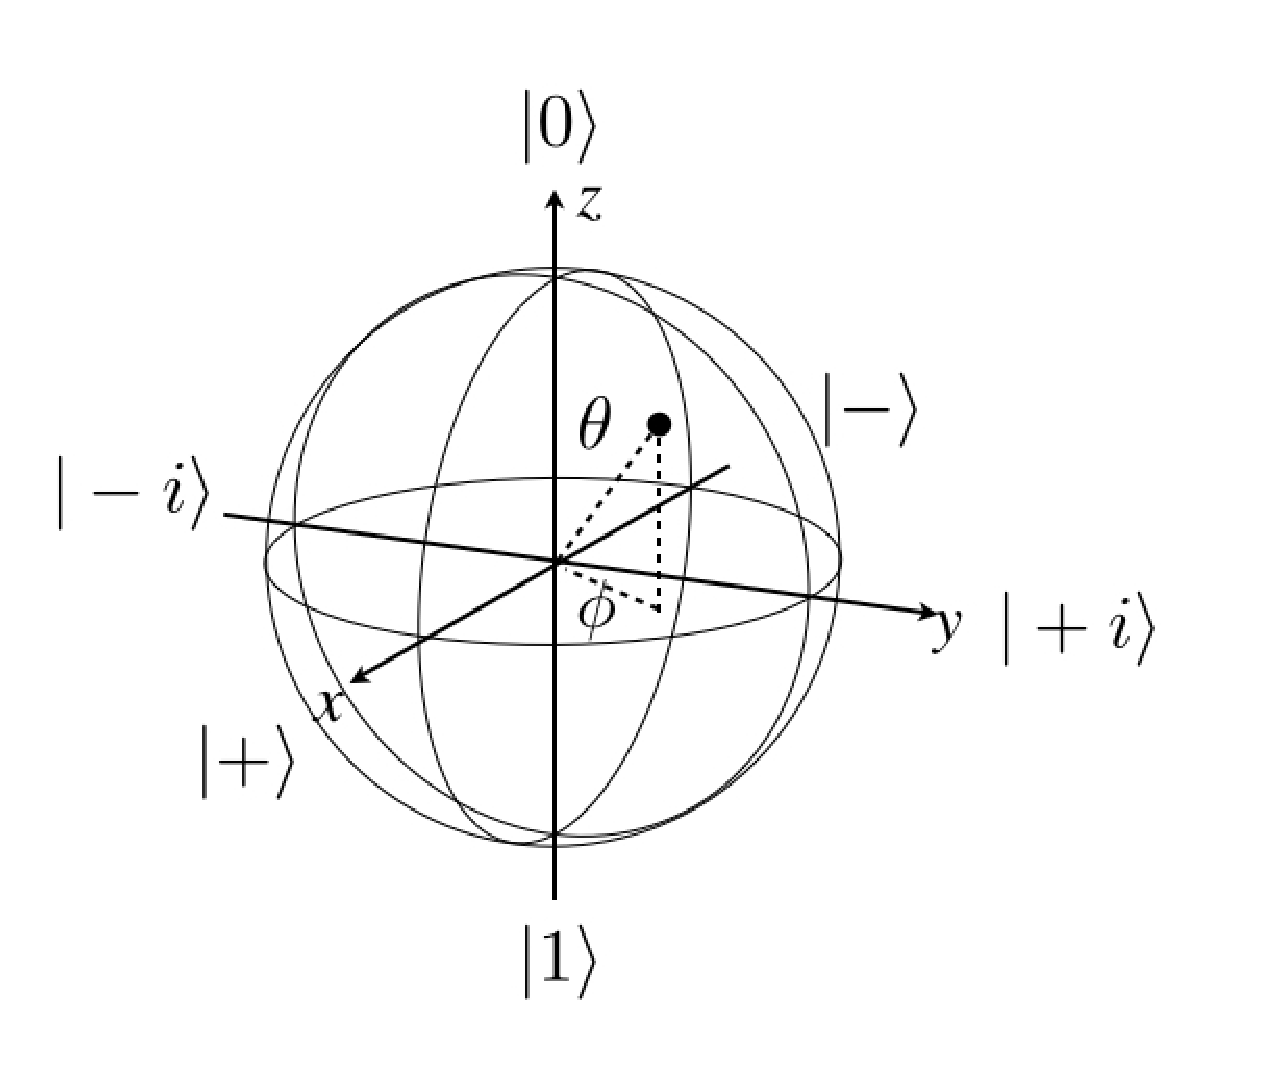
\includegraphics[width=100mm]{fig01.eps}
%
% If not, use
%\picplace{5cm}{2cm} % Give the correct figure height and width in cm
%
\caption{The Bloch sphere.}
\label{fig01}       % Give a unique label
\end{figure}


The time evolution, which maps a quantum state into another, is given as a unitary operator in quantum mechanics.
The most important operators are the Pauli operators\index{Pauli operator}
\begin{eqnarray}
I
=
\left(
\begin{array}{cc}
1 & 0
\\
0 & 1
\end{array}
\right),\ 
X
=
\left(
\begin{array}{cc}
0 & 1
\\
1 & 0
\end{array}
\right),\ 
Y
=
\left(
\begin{array}{cc}
0 & -i
\\
i & 0
\end{array}
\right),\ 
Z
=
\left(
\begin{array}{cc}
1 & 0
\\
0 & -1
\end{array}
\right).
\end{eqnarray}
The computational basis states $\{ |0\rangle , |1\rangle\}$ are eigenstates of the Pauli $Z$ operator.
The Pauli $X$ operator flips the computational basis state:
\begin{eqnarray}
|1\rangle = X|0\rangle, \;\;\; |0\rangle = X|1\rangle.
\end{eqnarray}
We define the eigenstates of the Pauli $X$ operator as
\begin{eqnarray}
|+\rangle = \frac{|0\rangle + |1\rangle}{\sqrt{2}},
\;\;\;
|-\rangle = \frac{|0\rangle - |1\rangle}{\sqrt{2}},
\end{eqnarray}
which we call the $X$-basis states.
Similarly, the eigenstates of the Pauli $Y$ operator are defined as 
\begin{eqnarray}
|+i\rangle = \frac{|0\rangle + i|1\rangle}{\sqrt{2}},
\;\;\;
|-i\rangle = \frac{|0\rangle - i|1\rangle}{\sqrt{2}},
\end{eqnarray}
which we call the $Y$-basis state.

The second most important operators are the Hadamard $H$ and phase $S$ operators
%
\begin{eqnarray*}
H=
\frac{1}{\sqrt{2}}
\left(
\begin{array}{cc}
1 & 1
\\
1 & -1
\end{array}
\right)
\textrm{ and }
S=
\left(
\begin{array}{cc}
1 & 0
\\
0 & i
\end{array}
\right).
\end{eqnarray*}
These gates transform between the different Pauli-basis states, i.e., $H: \{ |0\rangle , |1\rangle\} \leftrightarrow \{ |+\rangle, |-\rangle \}$ and
$S: \{ |+ \rangle , |-\rangle\} \leftrightarrow \{ |+i \rangle, |-i\rangle\}$.
Equivalently, we may say that these operators 
transform a Pauli operator into another Pauli operator under their conjugations:
\begin{eqnarray}
X=HZH, \;\;\; Y=SXS^{\dag}.
\end{eqnarray}
From this property, the $H$ and $S$ gates are called Clifford gates\index{Clifford gate}.
The Clifford gates are depicted as circuit diagrams as follows:
\begin{center}
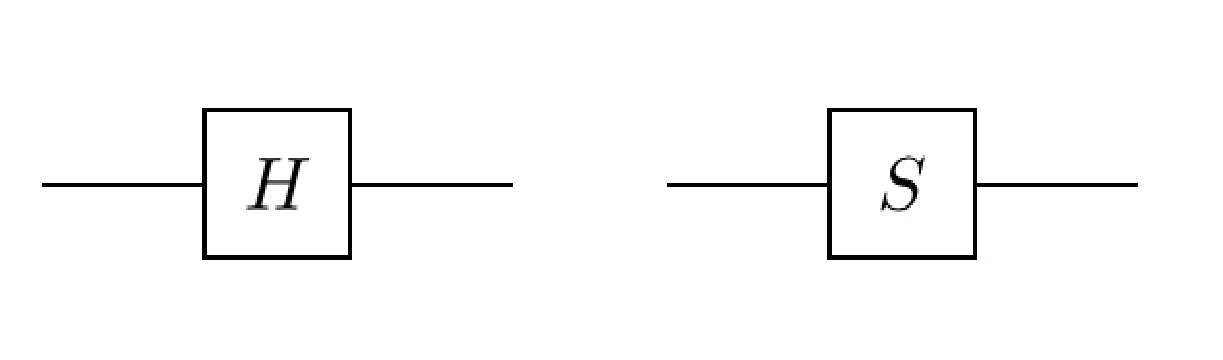
\includegraphics[width=100mm]{fig11.eps}
\end{center}

If we measure the qubit $|\psi \rangle$ in the $Z$-basis $\{ |0\rangle, |1\rangle \}$, we obtain the measurement outcomes 0 and 1 with probabilities 
\begin{eqnarray}
p_0 &=& |\langle 0 | \psi \rangle |^2 = {\rm Tr}\left[
|0\rangle\langle 0| \psi \rangle \langle \psi | \right] ,
\\
p_1 &=& |\langle 1 | \psi \rangle |^2 
= {\rm Tr}\left[|1\rangle\langle 1| \psi \rangle \langle \psi | \right],
\end{eqnarray}
respectively.
More generally, we may use the measurement operators $\{ M_i \}$, satisfying that $E_i \equiv M_i^{\dag}M_i$ is positive semidefinite and that $\sum _i E_i =I $.
(If an operator $A$ satisfies ${}^\forall |u\rangle$, $\langle u|A|u\rangle \geq 0$, it is said to be positive semidefinite.)
The probability of obtaining the measurement outcome $i$ is given by
\begin{eqnarray}
p_i = \langle \psi | M^{\dag}_i M_i | \psi \rangle 
= {\rm Tr} \left[ M^{\dag}_i M_i | \psi \rangle \langle \psi | \right]
= {\rm Tr} \left[ E_i | \psi \rangle \langle \psi | \right].
\end{eqnarray}
Such a measurement and the set of positive operators $\{ E_i = M_i ^{\dag} M_i\}$, are called a positive-operator-valued measure (POVM) measurement 
\index{positive-operator-valued measure measurement, POVM measurement} and POVM elements, respectively.
The post-measurement state conditioned on the measurement outcome $i$ is 
\begin{eqnarray}
\frac{M_i | \psi \rangle}{\sqrt{{\rm Tr} [ M^{\dag}_i M_i | \psi \rangle \langle \psi | ]}}.
\end{eqnarray}

Suppose we have quantum states $|\psi\rangle$ and $|\phi\rangle$ with probability $p_\psi$ and $p_{\phi}$, respectively.
We perform a measurement with the measurement operator $\{ M_i \}$.
If we assume that the measurement outcome $i$ is obtained with probability 
\begin{eqnarray}
p_i = p_{\psi} {\rm Tr} \left[ M^{\dag}_i M_i | \psi \rangle \langle \psi | \right]
+ p_{\phi} {\rm Tr} \left[ M^{\dag}_i M_i | \phi \rangle \langle \phi | \right],
\end{eqnarray}
we can express the classical mixture of $|\psi\rangle$ and $|\phi\rangle$ as an operator
\begin{eqnarray}
\rho =  p_\psi | \psi \rangle \langle \psi | + p_{\phi} | \phi \rangle \langle \phi |,
\end{eqnarray}
which is called the {\it density matrix} or {\it density operator}.
More generally, if we have pure quantum states $\{ |\psi _ k\rangle \}$ with probability $\{ p_{k}\}$, the density matrix is given by 
$\rho = \sum _k p_k | \psi \rangle \langle \psi |$.
A density matrix, which has information of a quantum state including its statistical property, has to be a positive hermitian (self-adjoint) operator $\rho$ satisfying 
${\rm Tr}\left[ \rho \right]=1$. 
Note that for a given density matrix $\rho$,
the pure state decomposition of it is not uniquely determined,
and any decomposition has the same statistical property.

A mixed state of a qubit $\rho$ can be represented as a point inside the Bloch sphere through the three coordinates calculated from the density matrix
\begin{eqnarray}
(r_x, r_y, r_z) = ( {\rm Tr}[X \rho],{\rm Tr}[Y \rho], {\rm Tr}[Z \rho] ).
\end{eqnarray}
If the state is a pure state $|\psi \rangle = \cos \frac{\theta }{2}|0\rangle+ e^{i \phi} \sin \frac{\theta}{2} |1\rangle$, the coordinates can be calculated to be
\begin{eqnarray}
(r_x, r_y, r_z) =(\sin \theta  \cos \phi,\sin \theta \sin \phi,\cos \theta ),
\end{eqnarray}
which is consistent with the previous definition.
The completely mixed state $I/2$ corresponds to the origin of the coordinate system.

\section{The Solovay-Kitaev algorithm}
The Pauli operators $\{I, X,Y,Z\}$ and single-qubit Clifford operators $\{H,S\}$ form a finite group, and hence cannot cover all unitary operations for a qubit.
If a non-Clifford operation exists, e.g., $e^{-i (\pi/8)Z}$, we can generate an arbitrary single-qubit unitary operation using the Solovay-Kitaev algorithm~\cite{DawsonNielsen05}.
The underlying Solovay-Kitaev theorem states that if a set of single-qubit operations generates a dense subset of $SU(2)$, then that set is guaranteed to fill $SU(2)$ quickly.

Suppose we have a basic ($0$th order) approximation $U_0$ of an arbitrary unitary operator $U$, and that it approximates $U$ with a certain constant error $\epsilon _0$:
\begin{eqnarray}
\Vert  U_0 - U \Vert  \leq \epsilon _0,
\end{eqnarray}
where $\Vert  ...\Vert $ indicates an operator norm.
The Solovay-Kitaev algorithm takes the $(n-1)$th order approximation $U_{n-1}$ with an error $\epsilon _{n-1}$ and returns the $n$th order approximation $U_n$ with an error $\epsilon _n$ as follows.

First, $U U^{\dag}_{n-1}$ is decomposed in terms of the unitary operators $V$ and $W$ as a group commutator:
\begin{eqnarray}
U U_{n-1}^{\dag}= VWV^{\dag}W^{\dag} ,
\label{eq:BGC}
\end{eqnarray}
where $V$ and $W$ are chosen such that 
\begin{eqnarray}
\Vert  V - I \Vert  < c \sqrt{\epsilon _{n-1}}, \;\;\; \Vert  W - I \Vert  < c \sqrt{\epsilon _{n-1}},
\end{eqnarray}
with a constant $c$.
The above decomposition always exists from the following argument.
Let $V$ and $W$ be rotations with an angle $\phi$ about the $x$- and $y$-axes, respectively.
Then $VWV^{\dag}W^{\dag}$ is a rotation with an angle $\theta$ about some axis, where
\begin{eqnarray}
\sin (\theta /2) = 2 \sin ^2 (\phi /2) \sqrt{1-\sin ^4 (\phi /2)}.
\end{eqnarray}
We assume that $\phi , \theta \ll 1$, and hence $\theta \simeq \phi^2$.
By inverting the above argument, if
\begin{eqnarray}
\Vert  I- VWV^{\dag}W^{\dag} \Vert  \simeq \theta /2 + O(\theta ^3)
\end{eqnarray}
we can find $V$ and $W$ such that
\begin{eqnarray}
\Vert  I - V\Vert  ,\;\; \Vert  I-W \Vert  \simeq \phi/2 + O(\phi^3).
\end{eqnarray}
Because
\begin{eqnarray}
\Vert I -U U_{n-1}^{\dag} \Vert  = \Vert  I- VWV^{\dag}W^{\dag} \Vert < \epsilon _{n-1},
\end{eqnarray}
we can find $V$ and $W$ such that $\Vert  I -V\Vert , \Vert I-W\Vert  <c \sqrt{\epsilon _{n-1}}$.

Second, we calculate the $(n-1)$th order approximations $V_{n-1}$ and $W_{n-1}$ of $V$ and $W$, respectively. 
Then the Solovay-Kitaev algorithm returns the $n$th order approximation 
\begin{eqnarray}
U_n = V_{n-1} W_{n-1} V^{\dag}_{n-1} W^{\dag}_{n-1} U_{n-1},
\end{eqnarray}
which satisfies 
\begin{eqnarray}
\Vert  U_n - U \Vert  \leq \epsilon _{n}.
\end{eqnarray}
Next, we will calculate $\epsilon _{n}$ as a function of $\epsilon _{n-1}$.
By using the property of the operator norm, we obtain 
\begin{eqnarray}
\Vert  U_n - U \Vert  &\leq &
\Vert V_{n-1} W_{n-1} V^{\dag}_{n-1} W^{\dag}_{n-1} - U U_{n-1}^{\dag} \Vert  \Vert  U_{n-1} \Vert 
\\
&\leq& 
\Vert V_{n-1} W_{n-1} V^{\dag}_{n-1} W^{\dag}_{n-1} - VWV^{\dag}W^{\dag} \Vert 
 \Vert  U_{n-1} \Vert 
\end{eqnarray}
By denoting
$V_{n-1} = V+ \Delta _V, \;\;\;  W_{n-1} = W+ \Delta _W$,
we obtain
\begin{eqnarray}
\Vert  U_n - U \Vert  &\leq & \Vert V_{n-1} W_{n-1} V^{\dag}_{n-1} W^{\dag}_{n-1} - VWV^{\dag}W^{\dag} \Vert 
 \\ &\leq &
\Vert   \Delta _V W V^{\dag} W^{\dag} 
+ VW  \Delta_V^{\dag} W^{\dag}   \Vert 
+
\Vert   V \Delta _W V^{\dag} W^{\dag} 
+  VW V^{\dag} \Delta_W^{\dag} \Vert 
+O(\Delta ^2).
\nonumber \\
\end{eqnarray}
Moreover, in terms of $\delta _V$ and $\delta _W$
defined by $V= I+ \delta _V$ and $W = W+ \delta _W$
respectively,
we obtain
\begin{eqnarray}
 \Vert  U_n - U \Vert  &\leq &
\Vert   \Delta _V  V^{\dag} 
+ V  \Delta_V^{\dag}    \Vert  
+
\Vert   \Delta _W  W^{\dag} 
+  W \Delta_W^{\dag} \Vert  
\\
&&
+ \Vert \Delta _V \delta _{W}\Vert 
+\Vert \Delta _V^{\dag} \delta _{W}^{\dag}\Vert 
+\Vert  \delta _V \Delta _W \Vert  + \Vert  \delta _V^{\dag} \Delta_W^{\dag}\Vert + O(\Delta ^2). 
\\ &\leq &
4 c\epsilon _{n-1}^{3/2}+O(\Delta ^2, \delta^2 \Delta) .
\end{eqnarray}
Here we have used that 
\begin{eqnarray}
\Delta _V  V^{\dag} 
+ V  \Delta_V^{\dag}   = \Delta _V \Delta _{V}^{\dag},
\end{eqnarray}
which can be derived from the unitarity of $V$ and $V_{n-1}=V+\Delta _V$.
To leading order, the error is given by $\epsilon _n \leq c' \epsilon _{n-1}^{3/2}$ with a certain constant $c'$ and is calculated to be 
\begin{eqnarray}
\epsilon _n \leq (2c' \epsilon _0)^{(3/2)^n}/(2c').
\label{eq:KSerror}
\end{eqnarray}
If $\epsilon _0 < 1/(2c')$, the error decreases super-exponentially in $n$.
On the other hand, the $n$th order approximation calls the $(n-1)$th order approximation three times, i.e., through $U_{n-1}$, $V_{n-1}$, and $W_{n-1}$.
Including the resource $R_D$ required for the decomposition (\ref{eq:BGC}), the overhead $R_n$ for the $n$th order approximation is given by
\begin{eqnarray}
&&R_n = 3R_{n-1} + R_D
\\
&\Leftrightarrow& R_n = O(3^n).
\label{eq:KSresource}
\end{eqnarray} 
Similarly, the number of unitary operations employed in the $n$th order approximation is calculated to be $M_n = O(5^n)$.
By using (\ref{eq:KSerror}) and (\ref{eq:KSresource}), the overhead $R_{\epsilon}$ and the number $M_{\epsilon}$ of gates required to obtain an approximation of $U$ with an error $\epsilon$ can be estimated: 
\begin{eqnarray}
R_{\epsilon} &=& O(\ln ^{\ln 3/\ln (3/2)} (1/\epsilon)),
\\
M_{\epsilon} &=& O(\ln ^{\ln 5/\ln (3/2)} (1/\epsilon)).
\end{eqnarray}
Thus, both $R_{\epsilon}$ and $M_{\epsilon}$ scale as polylogarithmic functions of $1/\epsilon$.


%%%%%%%%%%%%%%%%%%%%%%%%%%%%%%
%%%%%%%%%%%%%%%%%%%%%%%%%%%%%%%%%%%%%%%%%%%%%%%%%%%%%%%%%%%%
\section{Multi-qubit gates}
An $n$-qubit state is given by a superposition of tensor product states
\begin{eqnarray*}
| \Psi \rangle = \sum _{i_1 , i_2 ,... , i_n} C_{i_1 i_2 ... i_n} | i_1 i_2 ... i_n\rangle,
\label{eq01}
\end{eqnarray*}
where $i_k =0,1$ and $| i_1 i_2 ... i_n\rangle \equiv |i_1 \rangle \otimes |i_2 \rangle \otimes ... \otimes |i_n\rangle$.
A single qubit gate $A$ acting on the $k$th qubit is denoted by
\begin{eqnarray}
A_k = \overbrace{I \otimes \cdots \otimes I}^{k-1} \otimes A \otimes \overbrace{I \otimes \cdots I}^{n-k-1}.
\end{eqnarray}
An important two-qubit gate is the controlled-NOT (CNOT) gate,
\begin{eqnarray*}
\Lambda_{c,t} (X) = |0\rangle \langle 0| _{c} 
I_{t} + |1\rangle \langle 1|_{c}  X_{t}.
\end{eqnarray*}
For a computational basis input state $|i\rangle _{c} | j \rangle _{t}$, the CNOT gate acts as $\Lambda_{c,t}(X) |i\rangle _c |j \rangle _t = |i \oplus j \rangle$.
In this sense, the CNOT gate is a quantum generalization of the XOR operation in classical computation.
If the input state is $|+\rangle _{c} |0\rangle_{t}$, the output of the CNOT gate is a maximally entangled state:
\begin{eqnarray}
\Lambda _{c,t} (X) |+\rangle _{c}|0\rangle _{t} 
= (|00\rangle + |11\rangle )/\sqrt{2}.
\end{eqnarray}
The CNOT gate is depicted by a circuit diagram as follows:
\begin{center}
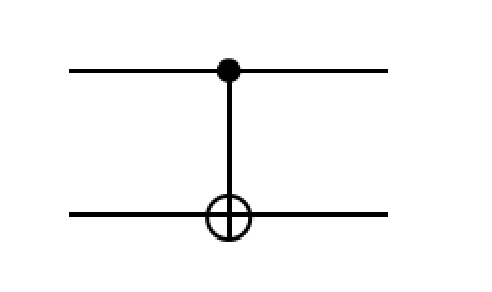
\includegraphics[width=50mm]{fig02.eps}
\end{center}

We may also define the controlled-$Z$ (CZ) gate,
\begin{eqnarray*}
\Lambda_{c,t} (Z) = |0\rangle \langle 0| _{c} 
I_{t} + |1\rangle \langle 1|_{c}  Z_{t}.
\end{eqnarray*}
The CZ operation is symmetric; $\Lambda _{c,t}(Z) = \Lambda _{t,c}(Z)$, and is represented by the circuit diagram
\begin{center}
\includegraphics[width=50mm]{fig03.eps}
\end{center}

Because the Pauli $Z$ operator is transformed into the Pauli $X$ operator by the Hadamard gate, we have the following relation between the CZ and CNOT gates:
\begin{center}
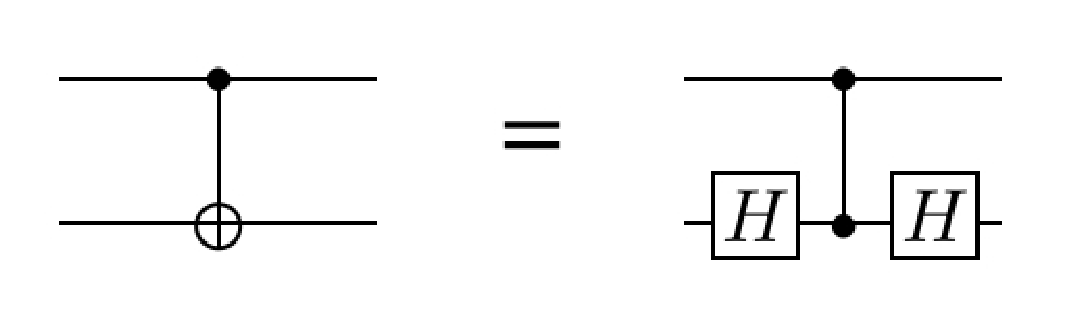
\includegraphics[width=100mm]{fig04.eps}
\end{center}


These CNOT and CZ gates are both Clifford gates, i.e., $\Lambda (A)$ ($A=X,Z$) transforms the two-qubit Pauli group onto itself under the conjugation 
$\Lambda (A) [ \cdots ] \Lambda (A)^{\dag}$.
For example,
$\Lambda (X) _{c,t} X_c \otimes I_t \Lambda (X) _{c,t}^{\dag} = X_c \otimes X_t$,
$\Lambda (X) _{c,t} I_c \otimes Z_t \Lambda (X) _{c,t}^{\dag} = Z_c \otimes Z_t$,
$\Lambda (Z) _{c,t} X_c \otimes I_t \Lambda (Z) _{c,t}^{\dag} = X_c \otimes Z_t$,
etc.

For an arbitrary unitary operator $U$, the controlled-$U$ gate is denoted by
\begin{eqnarray}
\Lambda _{c,t} (U) = |0\rangle \langle 0|_c I_t
+ |1\rangle \langle 1|_c  U_t,
\end{eqnarray}
where the qubits $c$ and $t$ are called the control and target qubits, respectively.
By decomposing a single-qubit unitary gate into $U=e^{ i \alpha }A X BXC$ with the unitary operators $A,B,C$ satisfying $ABC=I$, the controlled-$U$ operation $\Lambda(U)$ can be implemented as follows:
\begin{center}
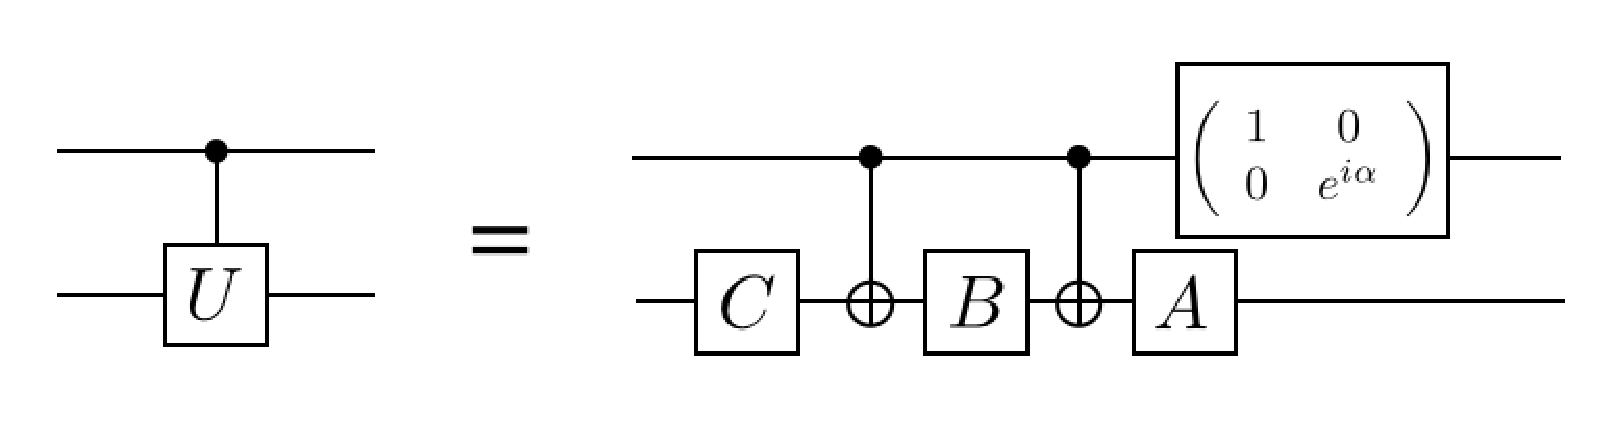
\includegraphics[width=120mm]{fig05.eps}
\end{center}
(Note that we always have such a decomposition for an arbitrary single-qubit 
gate~\cite{Barenco95,NielsenChuang}.)

For example, the controlled-Hadamard gate $\Lambda(H)$ can be represented by
\begin{center}
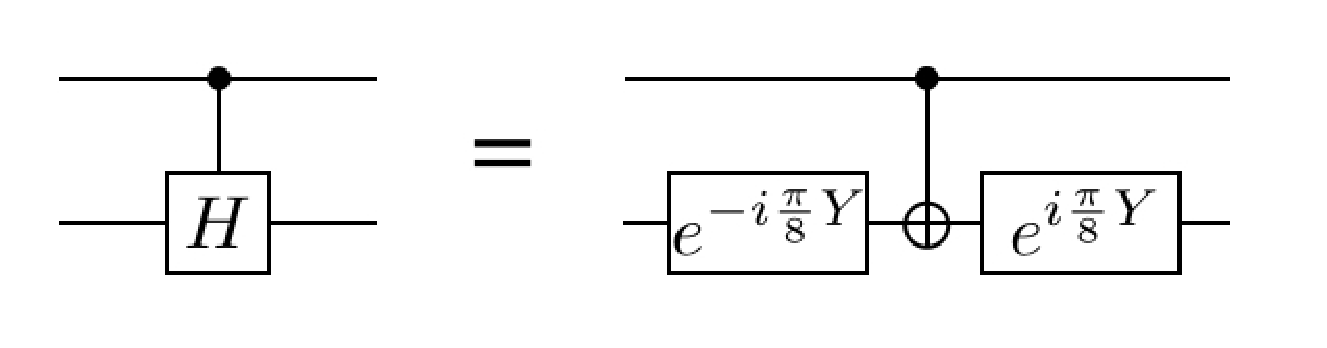
\includegraphics[width=100mm]{fig06.eps}
\end{center}


Next, we will discuss one of the most important multi-qubit gates, the Toffoli gate:
\begin{eqnarray}
\Lambda^2 _{c_1, c_2,t} (X) = (I_{c_1}I_{c_2} - |1\rangle \langle 1|_{c_1}|1\rangle \langle 1|_{c_2} ) I_{t} + |1\rangle \langle 1|_{c_1}|1\rangle \langle 1|_{c_2}   X_t,
\end{eqnarray}
which is depicted as a circuit diagram:
\begin{center}
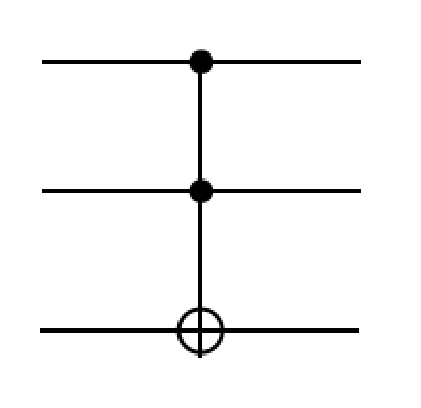
\includegraphics[width=30mm]{fig07.eps}
\end{center}
For a computational basis input state $|i_1\rangle _{c_1} |i_2 \rangle_{c_2} |j\rangle _{t}$, the Toffoli gate acts as
\begin{eqnarray}
\Lambda^2 _{c_1, c_2,t} (X)|i_1\rangle _{c_1} |i_2 \rangle_{c_2} |j\rangle _{t} = |i_1\rangle _{c_1} |i_2 \rangle_{c_2} |j\oplus (i_1 \cdot i_2) \rangle _{t}.
\end{eqnarray}
The state of the third qubit is equivalent to the output of the NAND operation in classical computation.
In this sense, the Toffoli operation can be regarded as a quantum extension of the NAND operation.
The NAND operations are known to be universal in classical computation in the sense that any logic gate (boolean function) can be constructed from them.
This implies that quantum computation trivially includes classical computation.
More importantly, because unitary operations are reversible, quantum computation can simulate classical computation in a reversible way.
Suppose we want to calculate a boolean function $f(x)$ for an input state $x$.
Then, we can construct a quantum circuit $U_f$ consisting of Toffoli and Pauli $X$ gates:
\begin{eqnarray}
U_f|x\rangle _{\rm input}|0...0\rangle _{\rm ancilla} |0\rangle_{\rm answer} = |x\rangle _{\rm input} |g(x) \rangle _{\rm ancilla} |f(x) \rangle_{\rm answer},
\end{eqnarray}
where the qubits $|\cdot\rangle_{\rm input}$, $|\cdot\rangle_{\rm ancilla}$, and $|\cdot\rangle_{\rm answer}$ indicate the registers for the input state, the ancillae for the Toffoli operations, and the answer of the calculation, respectively.
The output state of the ancilla register $|g(x)\rangle _{\rm ancilla}$ is the garbage of the computation.
However, the garbage can be uncomputed as follows (see also the circuit diagram below):
\begin{eqnarray}
&& U_f^{\dag} \Lambda _{\rm answer,out}(X) U_f|x\rangle _{\rm input}|0...0\rangle _{\rm ancilla} |0\rangle_{\rm answer} |0\rangle_{\rm out} 
\nonumber \\
&=& U_f^{\dag}|x\rangle _{\rm input} |g(x) \rangle _{\rm ancilla} |f(x) \rangle_{\rm answer} |f(x) \rangle_{\rm out}
\nonumber \\
&=&
|x\rangle _{\rm input} |0...0 \rangle _{\rm ancilla} |0 \rangle_{\rm answer} |f(x) \rangle_{\rm out}.
\end{eqnarray}
\begin{center}
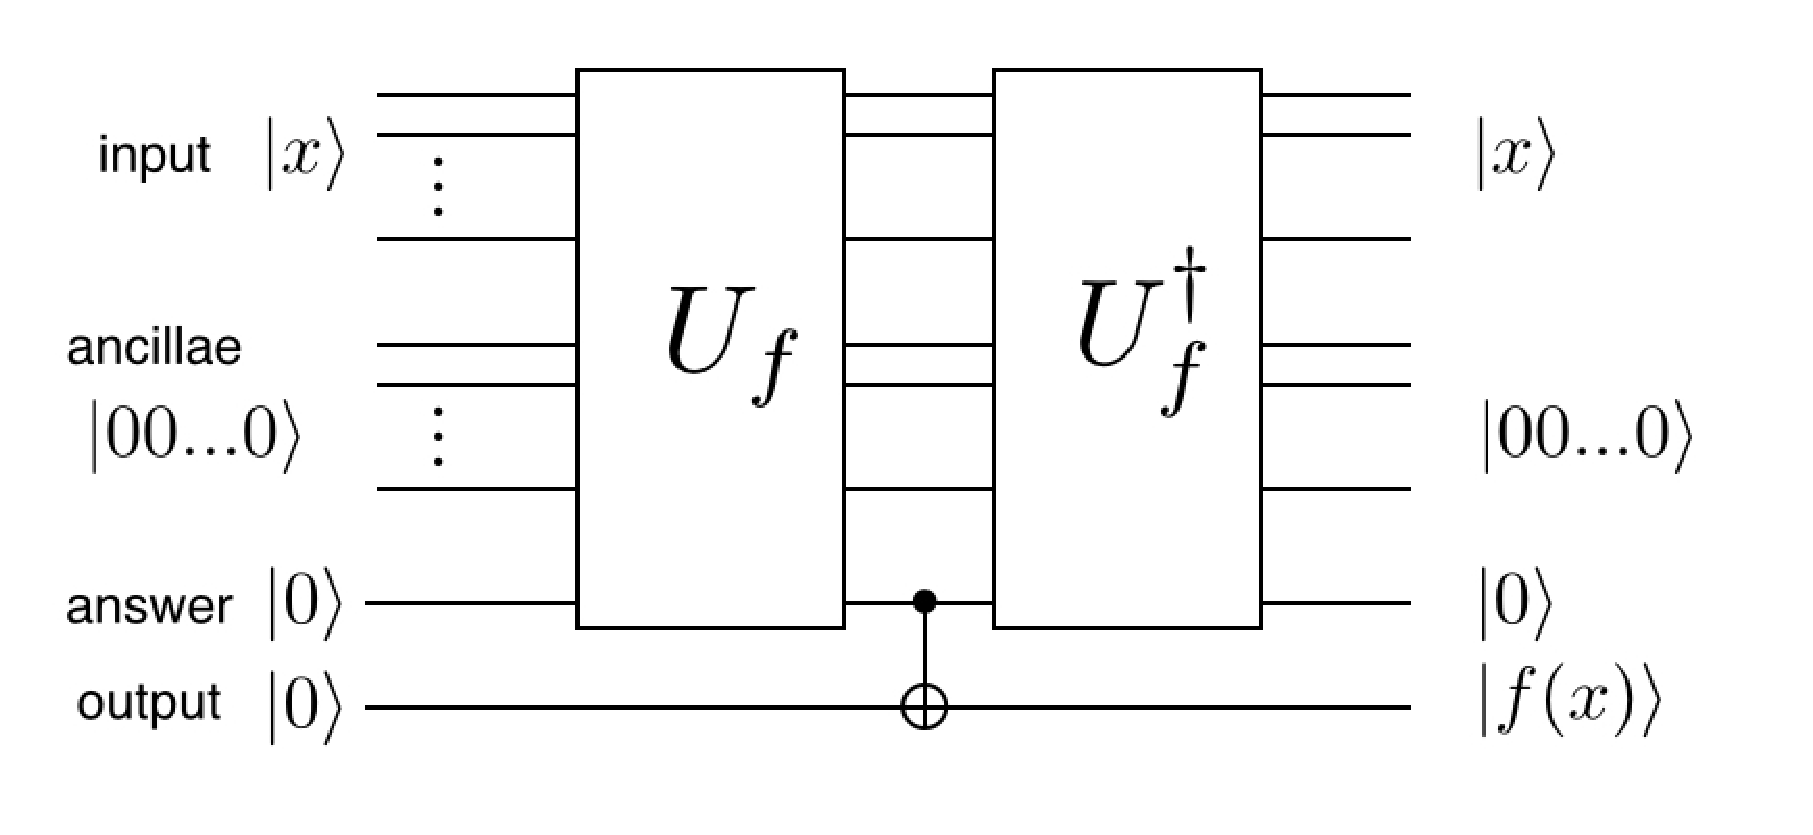
\includegraphics[width=110mm]{fig08.eps}
\end{center}
In this way, we can calculate an arbitrary boolean function in a reversible way.

Finally, we introduce the multi-controlled unitary gate
\begin{eqnarray}
\Lambda ^{k} (U) = (I^{\otimes k} - |1\rangle \langle 1|^{\otimes k}) \otimes I + |1\rangle \langle 1|^{\otimes k} \otimes U,
\end{eqnarray}
where $U$ is applied to the target qubit if all $k$ control qubits are $|1\rangle$.
The multi-controlled gate can be implemented by using the Toffoli gates and $k$ ancilla qubits as follow:
\begin{center}
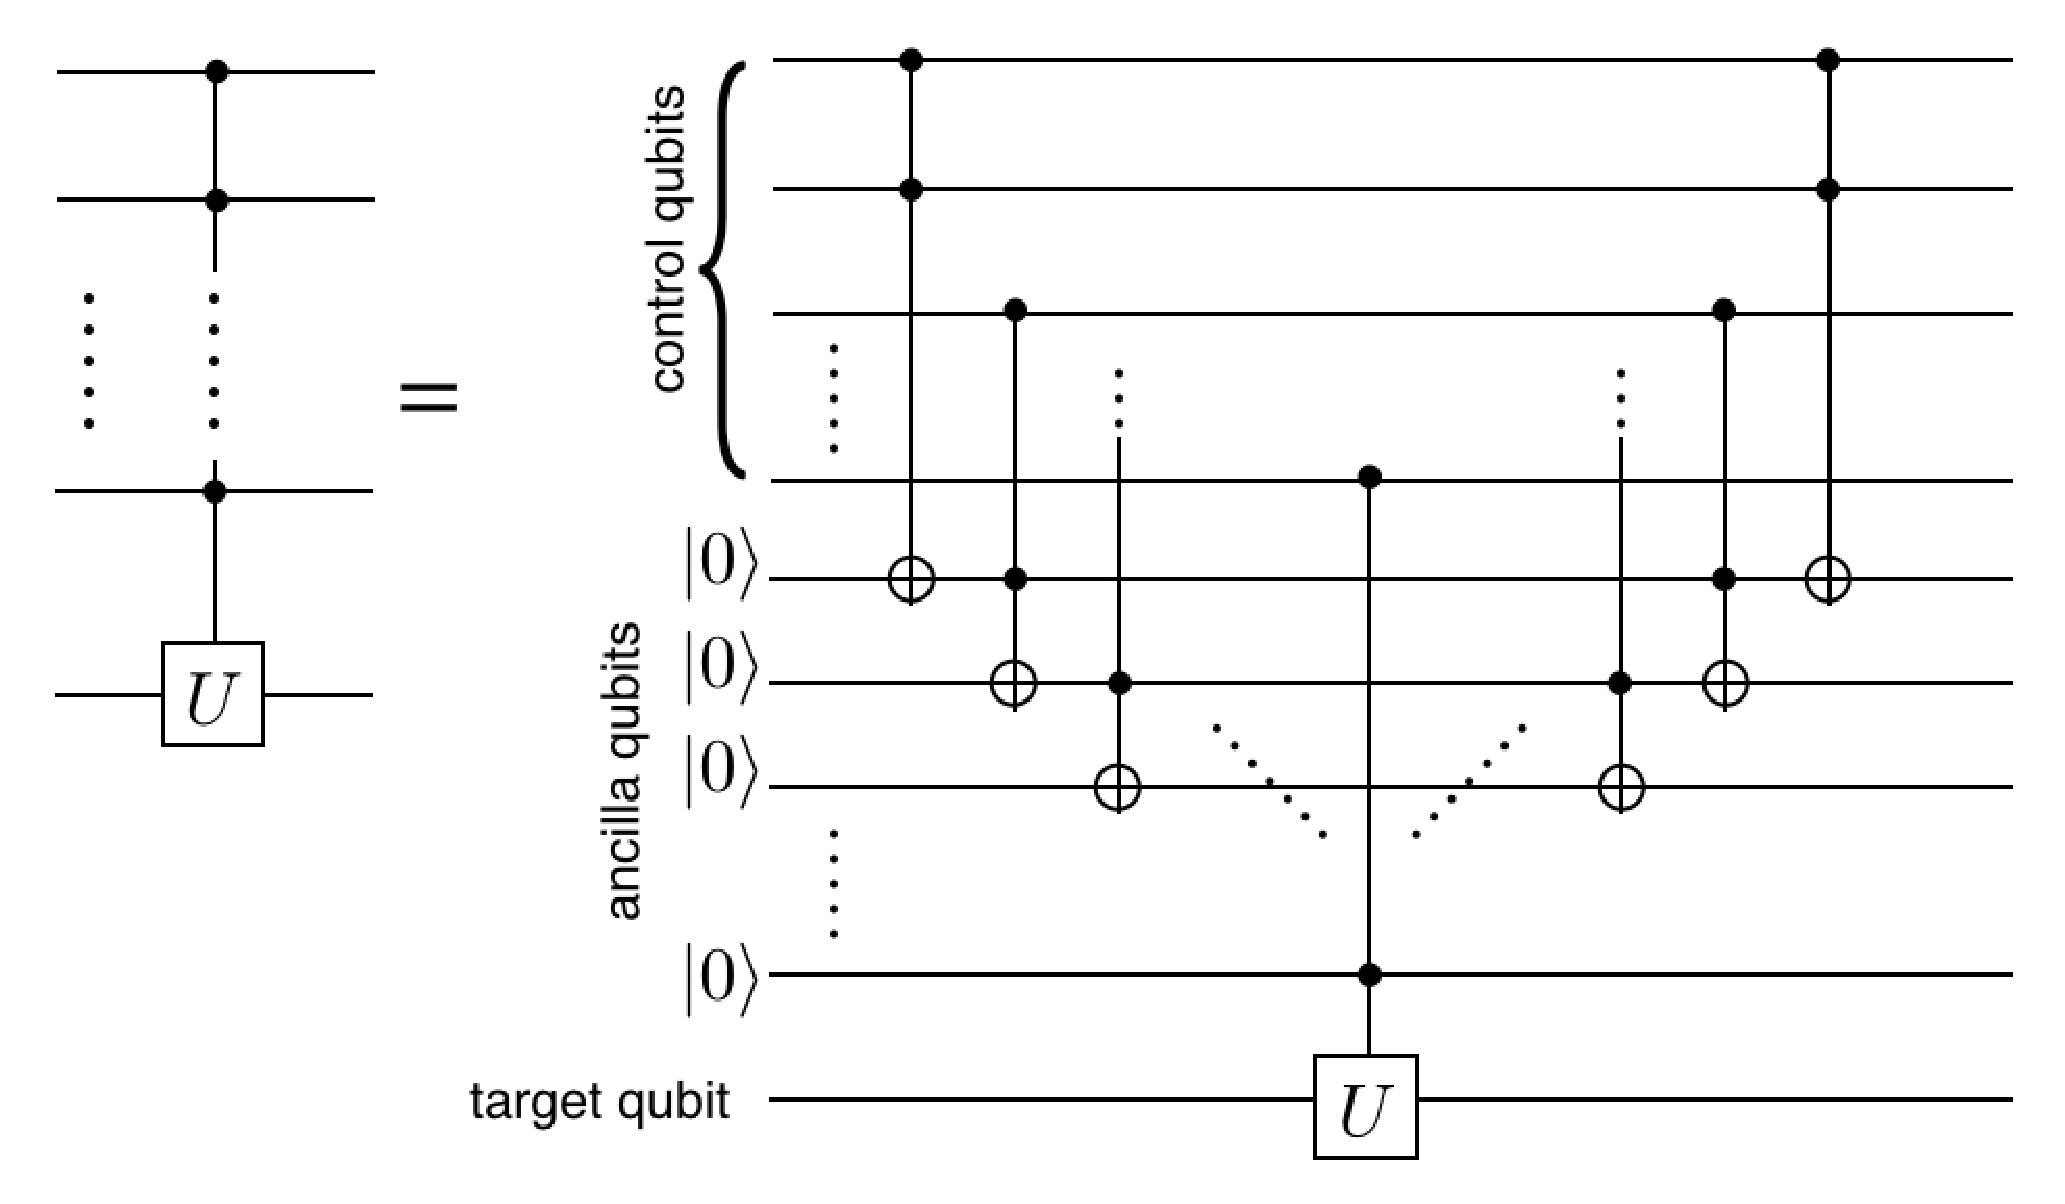
\includegraphics[width=110mm]{fig94.eps}
\end{center}
The $\Lambda ^2(U)$ gate can be decomposed into CNOT and single-qubit gates by using an idea similar to the decomposition of the $\Lambda (U)$ gate:
\begin{center}
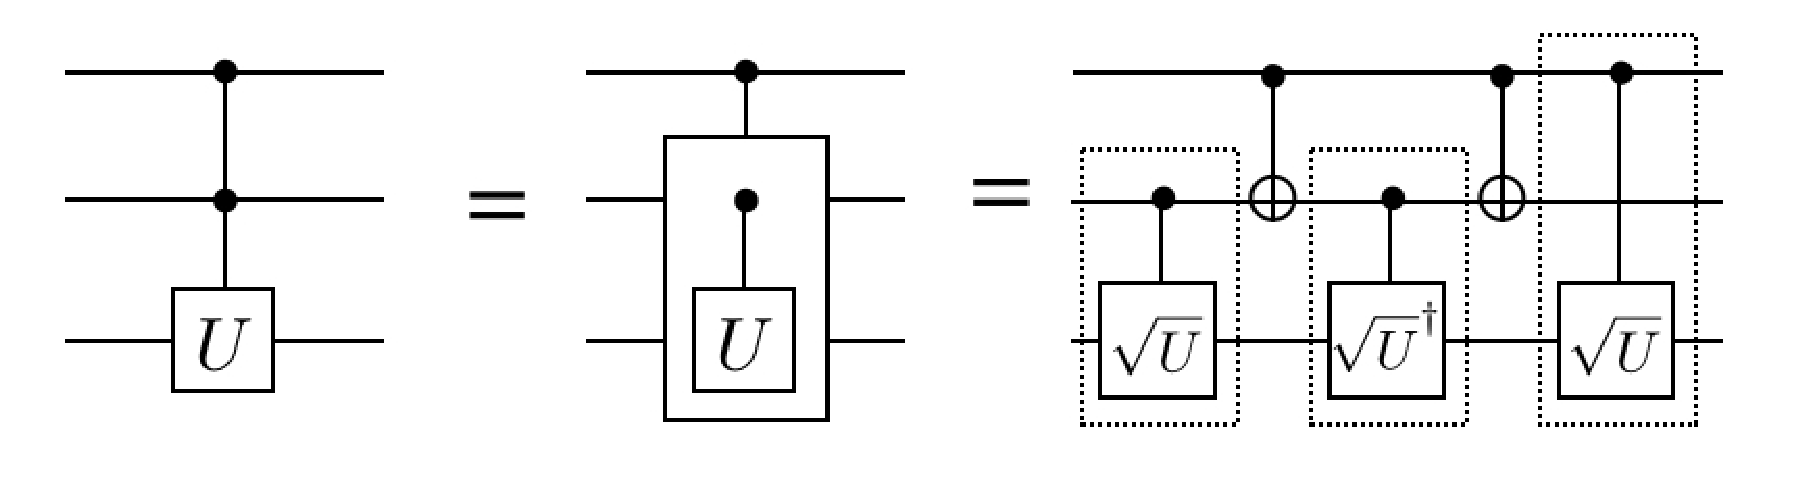
\includegraphics[width=100mm]{fig95.eps}
\end{center}
For example, the Toffoli gate can be constructed from the CNOT, Hadamard, and $\pi/8$ operations as follows: 
\begin{center}
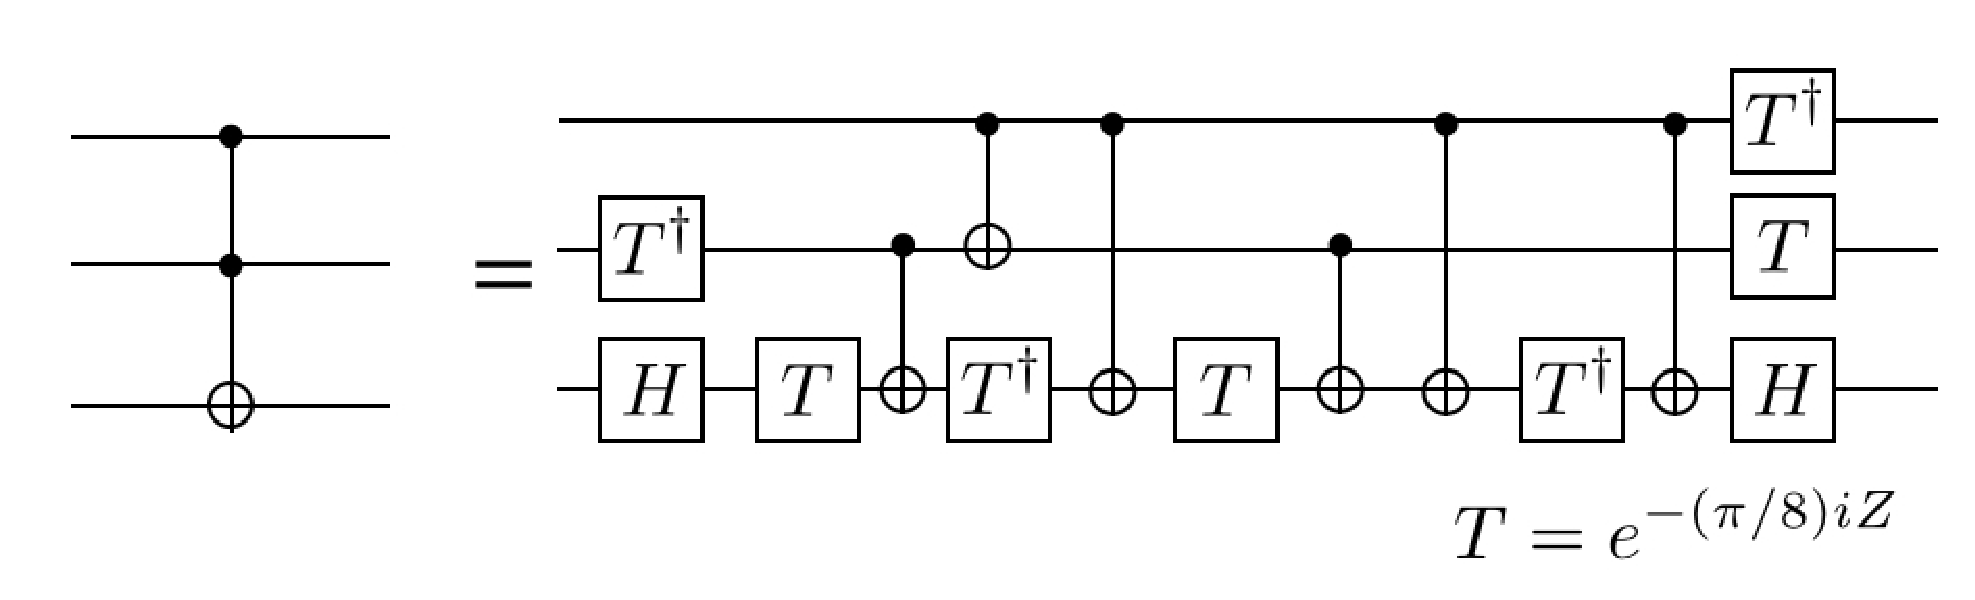
\includegraphics[width=100mm]{fig09.eps}
\end{center}
where we have used the fact that that the controlled-$\sqrt{X}$ gate is decomposed into the CNOT, Hadamard, and $\pi/8$ ($T= e^{-i (\pi/8)Z}$) gates as follows:
\begin{center}
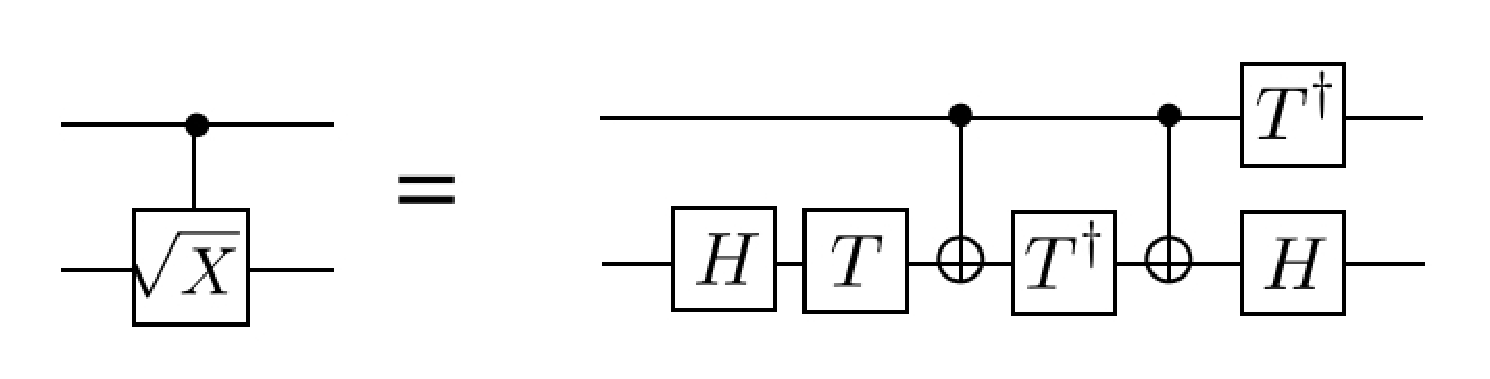
\includegraphics[width=80mm]{fig97.eps}
\end{center}
It should be noted that
a multi-controlled gate $\Lambda ^k (U)$
can also be constructed
without any ancilla qubit 
from multi-controlled gates $\Lambda ^{(k-1)} (U)$ 
with lower controlled qubits
by using the trick employed for decomposing 
$\Lambda ^2(U)$ into $\Lambda (U)$~\cite{Barenco95}.



\section{Universal quantum computation}
Here we will show that an arbitrary unitary operation 
can be decomposed into single-qubit and CNOT gates.
To this end, we will first show how to decompose an arbitrary unitary operation into a product of two-level unitary gates.
Second, the two-level gates are decomposed into 
the multi-controlled gates,
which can be constructed from single-qubit and CNOT gates
as seen in the previous section.

Let $U$ be an arbitrary $n$-qubit unitary operator, represented by an $m\times m$ unitary matrix with $m\equiv 2^n$.
Let $T_{ij}$ be a unitary operator such that $(T_{ij})_{kl} = \delta _{kl}$ if $k,l \neq i,j$, which we call a two-level unitary gate.
(The $kl$ element of a matrix $A$ is denoted by $(A)_{kl}$.)
The $ii$, $ij$, $ji$, and $jj$ elements define a unitary operation on the two-level subsystem spanned by $|j\rangle$ and $|i\rangle$.
By choosing $T_{m\; m-1}$ appropriately, we have
\begin{eqnarray}
U T_{m \;m-1} = \left( 
\begin{array}{cccc}
	u_{11} & \cdots & u_{1\; m-1} & u_{1 \; m}
\\
	\vdots & \ddots & \vdots & \vdots
\\
	u_{m-1 \; 1} & \cdots & u'_{m-1 \; m-1} & u'_{m-1 \; m}
\\
	u_{m \; 1} & \cdots & 0  & u'_{m \; m}
\end{array}
\right),
\end{eqnarray}
where $(U)_{kl} = u_{kl}$.
By repeating this procedure, we obtain 
\begin{eqnarray}
U T_{m \; m-1} T_{m \; m-2} \cdots T_{m \; 1} 
= 
\left(
\begin{array}{cccc}
	u''_{11} & \cdots & u''_{1\; m-1} & u''_{1 \; m}
\\
	\vdots & \ddots & \vdots & \vdots
\\
	u''_{m-1 \; 1} & \cdots & u''_{m-1 \; m-1} & u''_{m-1 \; m}
\\
	0 & \cdots & 0  & u''_{m \; m}
\end{array}
\right).
\end{eqnarray}
Due to unitarity, $u'' _{1\;m}=\cdots = u''_{m-1 \; m}=0$ and $|u''_{mm}|=1$.
Defining $R_{m} \equiv T_{m \; m-1} T_{m \; m-2} \cdots T_{m \; 1} $, we can decompose $U$ into a product of $R_k$ and a diagonal unitary operator $D$:
\begin{eqnarray}
U= D (R_{m} \cdots R_1)^{\dag}.
\end{eqnarray}
It is obvious that $D$ can be decomposed into two-level unitary gates.
Thus, an arbitrary unitary operator $U$ can be decomposed into two-level unitary gates.

Next, we show that any two-level unitary operator $T_{ij}$ can be implemented by using CNOT and single-qubit gates.
Let us rewritte $i$ and $j$ ($i,j= 0,..., m-1$) by using the $n$-bit strings $\mathbf{s}=s_1 s_2 ... s_n$ and $\mathbf{t}=t_1 t_2 ... t_n$, respectively.
It is easy to find a sequence of $n$-bit strings $\{ \mathbf{g}_{k} \}_{k=1}^{d}$ such that $\mathbf{s}=\mathbf{g}_1$, $\mathbf{t}=\mathbf{g}_{d}$, and $\mathbf{g}_k$ and $\mathbf{g}_{k+1}$ differ by only one bit.
By using the Pauli $X$ gate and the multi-controlled-NOT gate
controlled by the same $n-1$ bits and targeting the one different bit,
we can transform the basis $|\mathbf{g}_k\rangle$ to $|\mathbf{g}_{k+1}\rangle$.
In this way, the basis $| i \rangle = |\mathbf{s}\rangle = |\mathbf{g}_1\rangle$ is transformed into $|\mathbf{g}_{d-1}\rangle$.
After this basis transformation, we now want to apply a two-level unitary gate between $|\mathbf{g}_{d-1}\rangle$ and $|j\rangle =|\mathbf{t}\rangle = |\mathbf{g}_{d}\rangle$.
Because $\mathbf{g}_{d-1}$ and $\mathbf{g}_{d}$ differ by only one bit, we can perform such a two-level unitary gate by the multi-conditional gate, using the Pauli $X$ gate for bit flips.
Finally, the basis $|\mathbf{g}_{d-1}\rangle$ is returned to $|\mathbf{s}\rangle$ by applying the inverse of the basis transformation.

For example, a two-level unitary operator acting on a subspace spanned by $\{ |000\rangle , |111\rangle\}$ can be implemented as follows:
\begin{center}
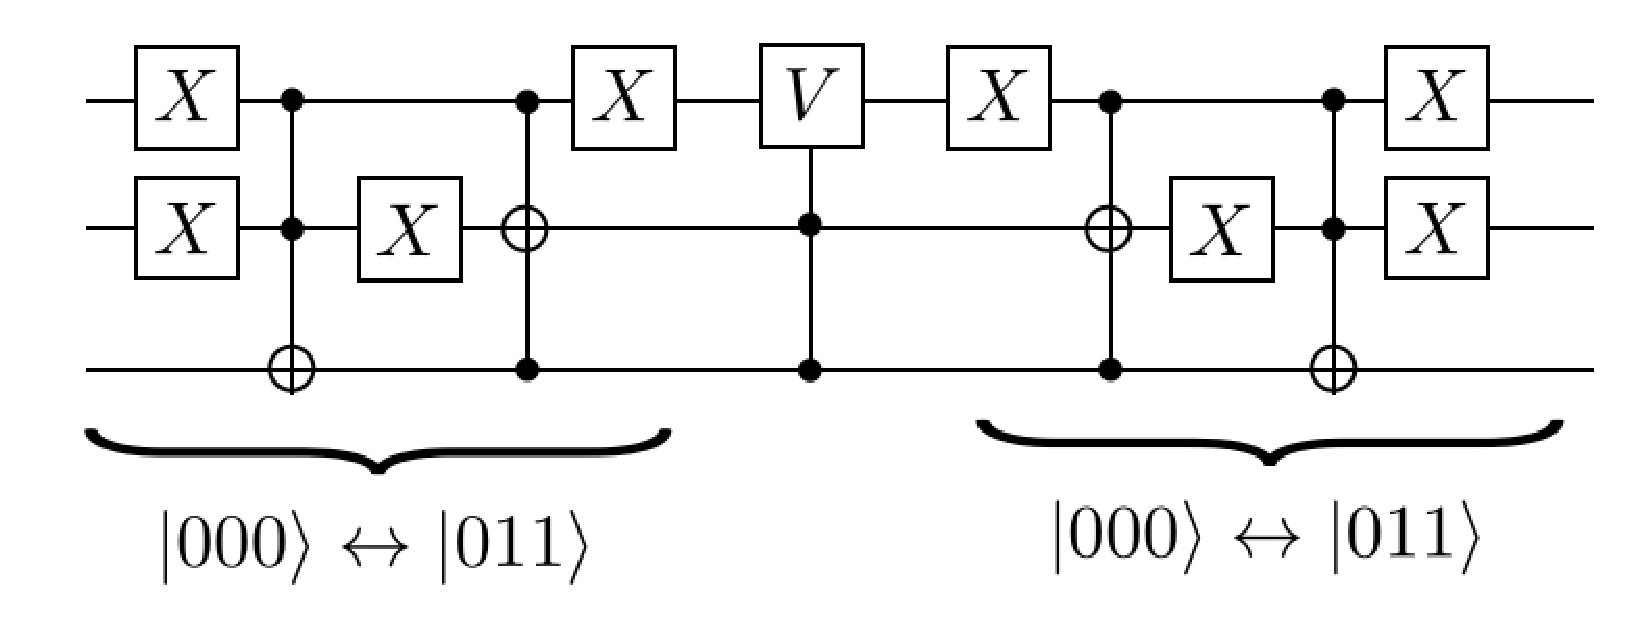
\includegraphics[width=120mm]{fig10.eps}
\end{center}

As seen previously, the multi-conditional gate can be decomposed into CNOT and single-qubit gates.
Moreover, an arbitrary single-qubit unitary operation can be approximated by using the Hadamard and $\pi/8$ operations by virtue of the Solovay-Kitaev algorithm.
Thus, the CNOT, Hadamard, and $\pi/8$ operations form a universal set of operations for quantum computations.
The Toffoli and Hadamard operations also form a universal set as shown in~\cite{Reck94,Barenco95,DiVincenzo95,BernsteinVazirani,NielsenChuang}. 

\section{Quantum algorithms}
\label{sec:Qgadget}
In this section, we explain two representative quantum algorithms; Shor's prime factorization algorithm~\cite{Shor,Shor97} and the Aharonov-Jones-Landau algorithm for an additive approximation of the Jones polynomial~\cite{AharonovJones,AharonovJonesHard}.
We do not go deep into the mathematically rigorous details, but we aim to understand how they work.
The readers who are interested in more details should read Refs.~\cite{Shor,Shor97,KitaevAbelian,NielsenChuang,AharonovJones,AharonovJonesHard}.

\subsection{Indirect measurement and the Hadamard test}
\label{sec:HadamardTest}
An indirect measurement of an observable (hermitian) $A$ with eigenvalues $\pm 1$ can be performed by using $\Lambda(A)$:
\begin{center}
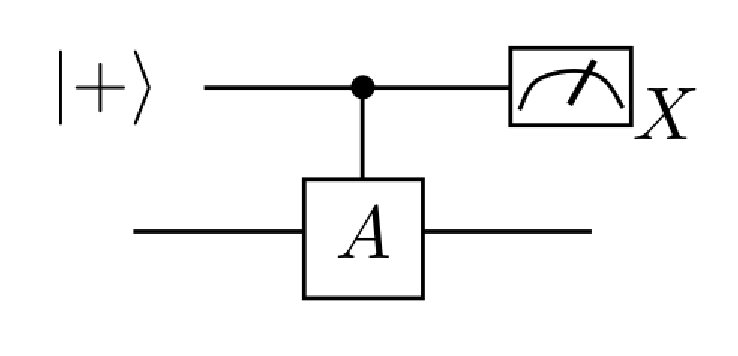
\includegraphics[width=50mm]{fig12.eps}
\end{center}
By denoting the input state $|\psi \rangle$, the post-measurement state is given by
\begin{eqnarray}
\frac{I+(-1)^{s}A}{2}|\psi \rangle /\sqrt{{\rm Tr}[(I+(-1)^s A)/2|\psi \rangle \langle \psi | ]},
\end{eqnarray}
where $s=0,1$ is the measurement outcome.
For example, a circuit measuring the eigenvalue of the operator $X_1X_2X_3$ is given by
\begin{center}
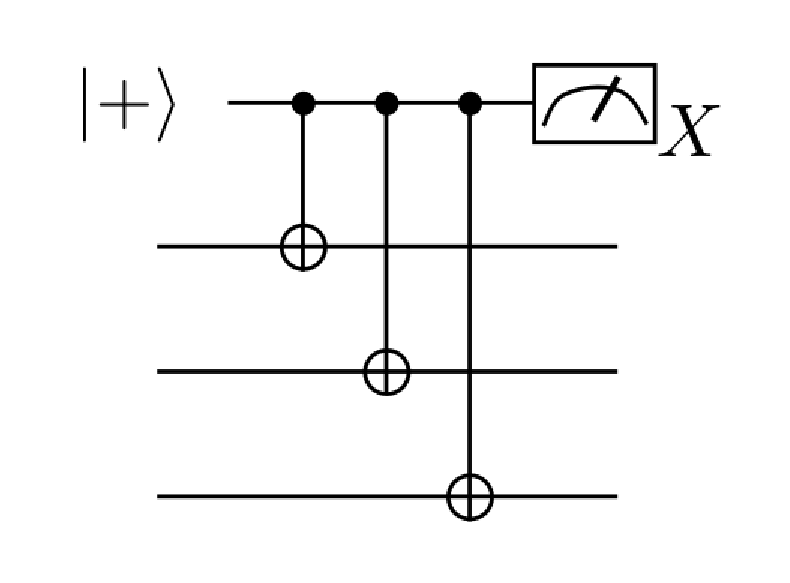
\includegraphics[width=50mm]{fig16.eps}
\end{center}
According to the measurement outcome $s=0,1$, the post-measurement state is projected by $\frac{I +(-1)^{s}X_1 X_2 X_3}{2}$.
The indirect measurement will be employed frequently in quantum error correction to measure the eigenvalues of the stabilizer operators.

%\subsubsection{Hadamard test}
The Hadamard test\index{Hadamard test} of an arbitrary unitary operator $U$ is defined by the following circuit:
\begin{center}
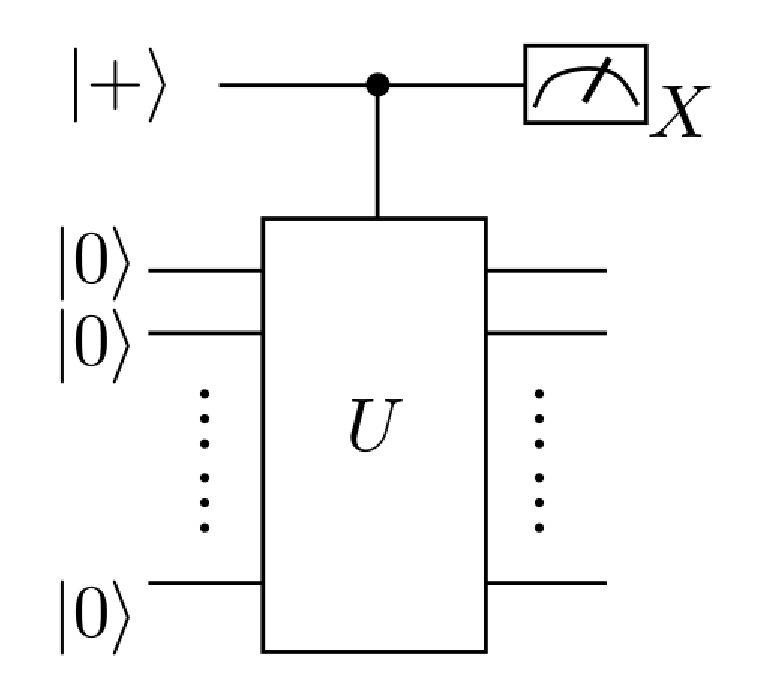
\includegraphics[width=50mm]{fig13.eps}
\end{center}
The probabilities of the measurement outcomes $0,1$ of the $X$-basis measurement are calculated to be
\begin{eqnarray}
p_0 &=& \frac{1}{2}\left( 1+ {\rm Re} \langle 0 | ^{\otimes n} U |0 \rangle ^{ \otimes n}\right),
\\
p_1 &=& \frac{1}{2}\left( 1- {\rm Re} \langle 0 | ^{\otimes n} U |0 \rangle ^{ \otimes n}\right).
\end{eqnarray}
Similarly, the Hadamard test for the imaginary part is defined:
\begin{center}
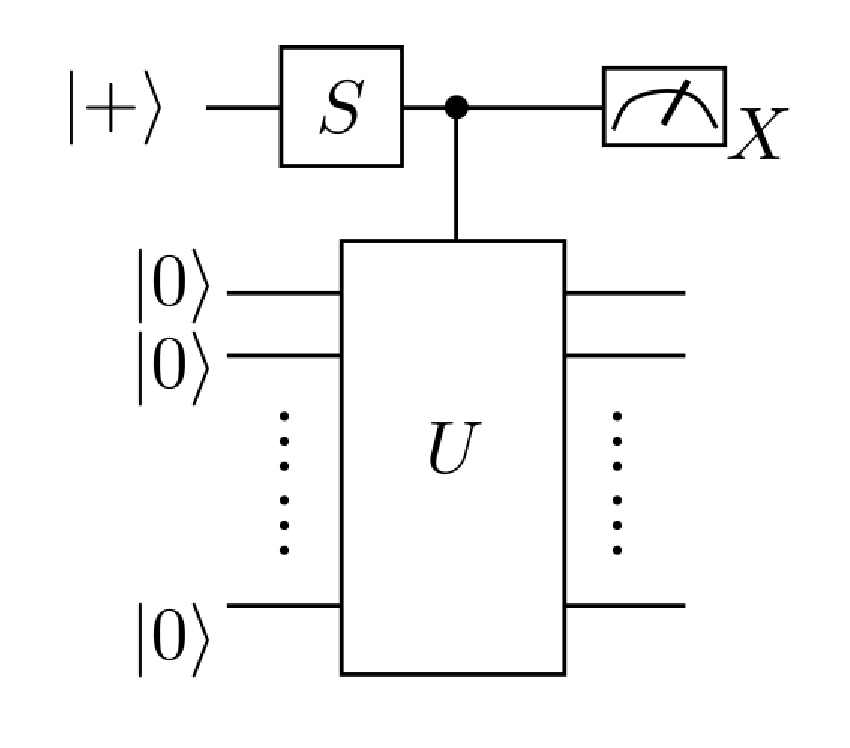
\includegraphics[width=55mm]{fig14.eps}
\end{center}
Suppose we perform the Hadamard test $N$ times and obtain the measurement outcome 0, $N_0$ times.
By using the Chernoff-Hoeffding bound\index{Chernoff-Hoeffding bound},
\begin{eqnarray}
{\rm Prob} \left( \left| \frac{N_0}{N} - p_0\right| > \epsilon \right) < 2 e^{-2 \epsilon ^2 N},
\end{eqnarray}
we can estimate the matrix element $\langle 0 | ^{\otimes n} U |0 \rangle ^{ \otimes n}$ with an error $\epsilon$ by repeating the Hadamard test $N={\rm poly}(1/\epsilon)$ times.
The Hadamard test is employed in various quantum algorithms such as approximations of the Jones and Tutte polynomials~\cite{AharonovJones,AharonovJonesHard,AharonovTutte} and the partition functions of statistical mechanical models~\cite{Cuevas11,Iblisdir,MatsuoFujii}.

Specifically, if we choose the input state to be a completely mixed $n$-qubit state,
\begin{center}
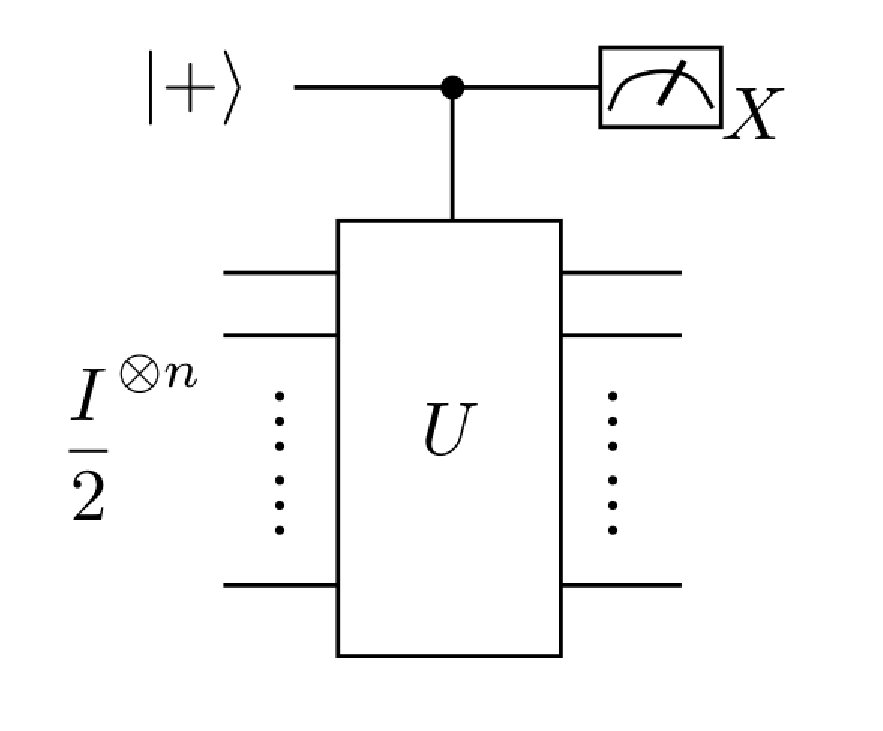
\includegraphics[width=55mm]{fig15.eps}
\end{center}
then, the Hadamard test provides the trace ${\rm Tr}[U]/2^n$ of the unitary operator $U$.
Such a restricted type of quantum computation is called a deterministic quantum computation with one clean qubit (DQC1) \index{deterministic quantum computation with one clean qubit, DQC1}~\cite{DQC1}.
DQC1 seems to be less powerful than universal quantum computation, because only one qubit is a pure state.
% entanglement is bounded
However, DQC1 can evaluate functions, which would be intractable on a classical computer, such as the Jones and Homefly polynomials~\cite{ShorJordan,JordanWacjan}, spectral density function~\cite{DQC1}, and fidelity decay~\cite{FidelityDecay}.
Recently, classical sampling of the output of DQC1 with a few qubits measurements has been shown to be intractable unless the polynomial hierarchy collapses to the third level~\cite{DQC1hardness,DQC12}.

\subsection{Phase estimation, quantum Fourier transformation, and factorization}
\index{Shor's factorization algorithm}
If we have an eigenstate $|E_i\rangle$ of a unitary operator $U$, for which $\Lambda (U)$ is described by a polynomial number of gates, we can estimate the eigenvalue $\lambda _i$ of $U$ with a polynomial accuracy using the Hadamard test as follows:
\begin{center}
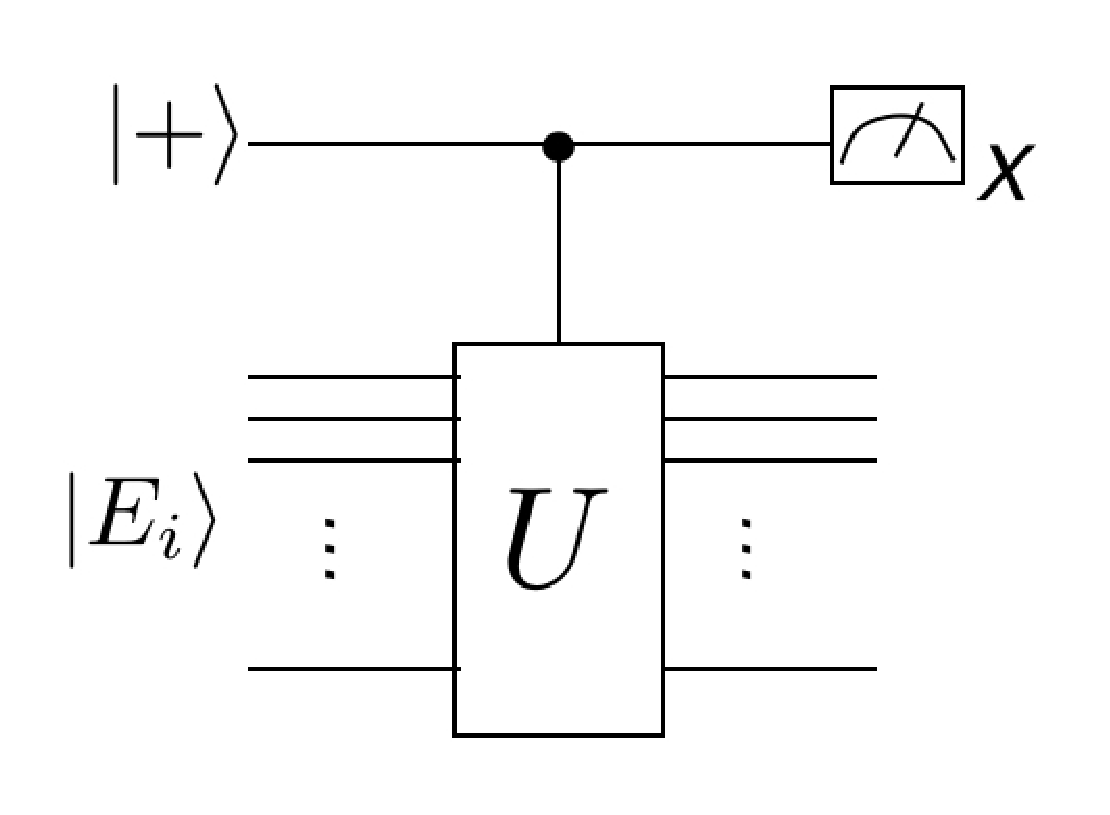
\includegraphics[width=60mm]{fig90.eps}
\end{center}
When we do not have the eigenstate, the input state is projected onto one of the eigenstates by the Hadamard test.
Thus, by repeating the Hadamard test, we can obtain one of the eigenvalues with polynomial accuracy.

Moreover, if a controlled-$U^{2^k}$ gate $\Lambda (U^{2^k})$ can be described by a polynomial number of gates, we can estimate the eigenvalue with exponential accuracy~\cite{KitaevPhase}.
Suppose the eigenvalue is given by $\lambda _i =e^{i \phi}=e^{2 \pi i 0.j_1 j_2 ... j_n} $, where we employ a decimal of a binary number,
\begin{eqnarray}
0.j_1 j_2 ... j_n = \sum _{k=1}^{n} j_k (1/2)^k.
\end{eqnarray}
Then, the Kitaev's phase estimation algorithm\index{Kitaev's phase estimation algorithm} is given by 
\begin{center}
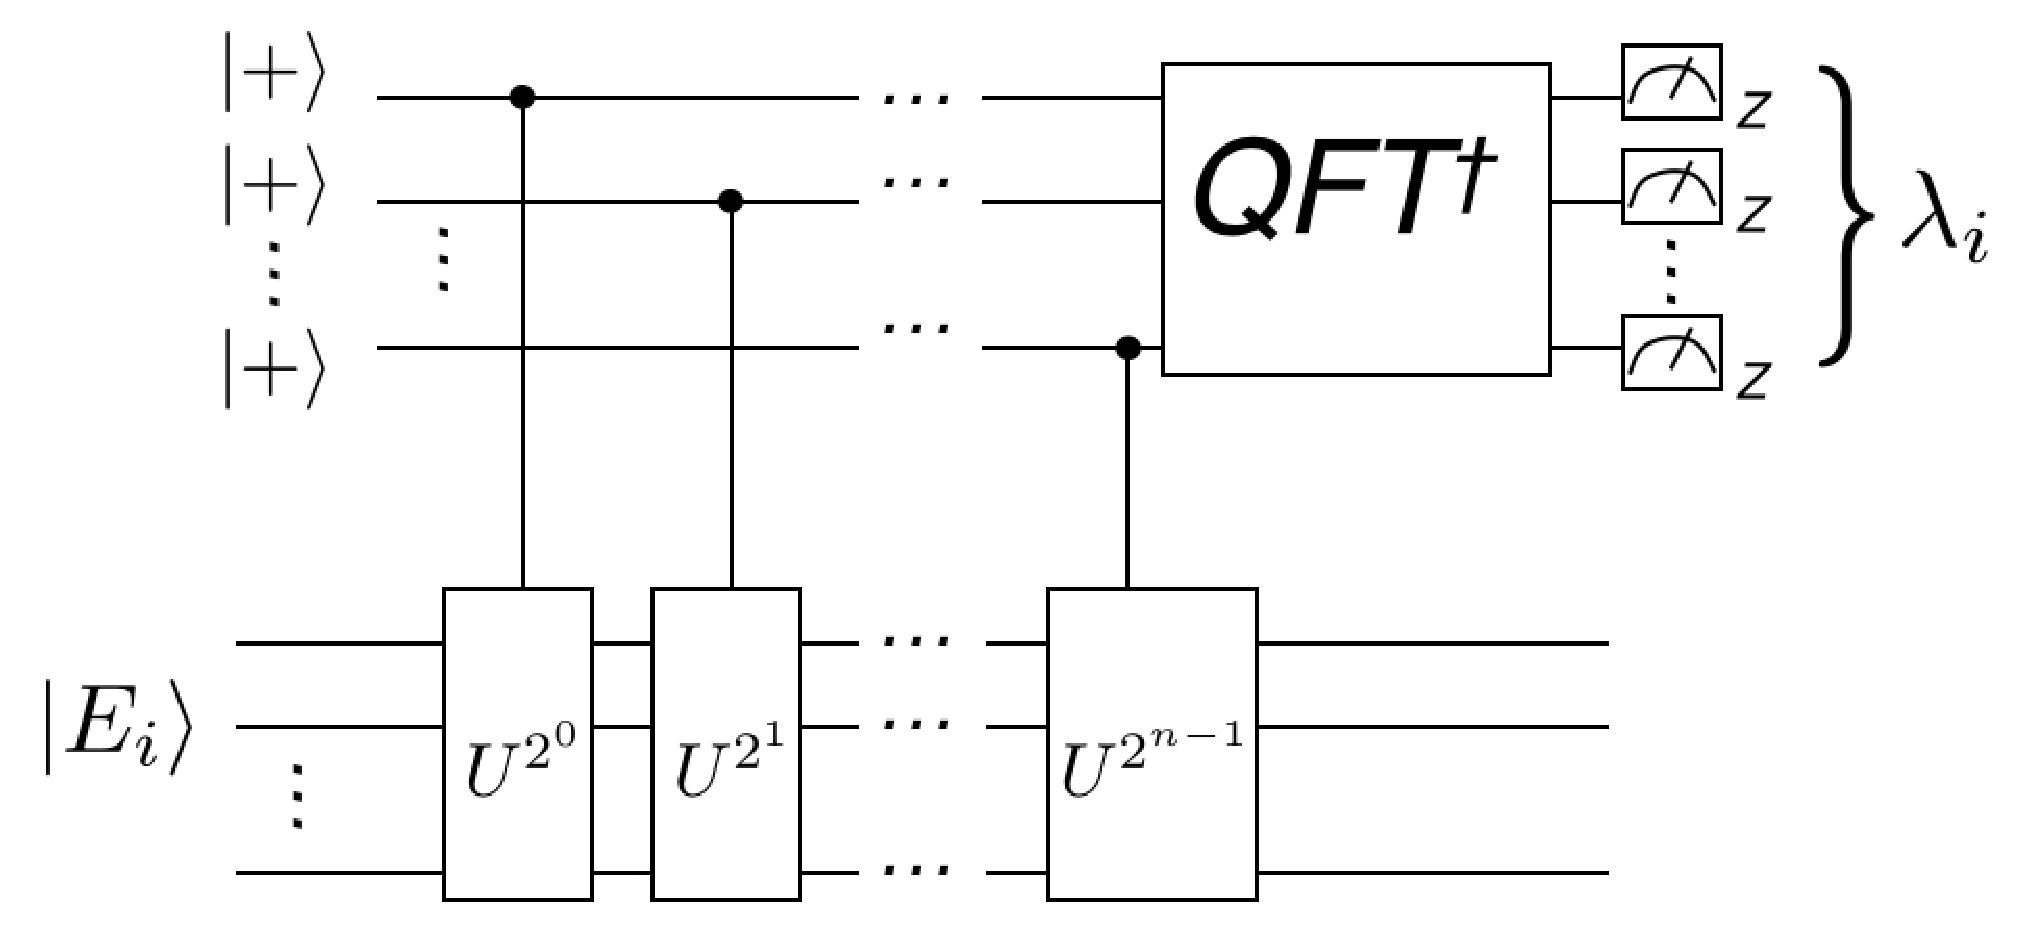
\includegraphics[width=110mm]{fig91.eps}
\end{center}
where QFT stands for the quantum Fourier transform\index{quantum Fourier transform}.
The controlled gate $\Lambda (U^{2^k})$ kicks back the phase $e^{2^k \phi}=e^{2 \pi i j_k.j_{k+1}...  j_n}$ to the ancilla state $|+\rangle$.
The phase information is transformed into a computational basis state by using the inverse quantum Fourier transformation:
\begin{eqnarray}
QFT^{\dag} (|0\rangle + e^{2\pi i 0.j_1 j_2 ... j_n }|1\rangle)
(|0\rangle + e^{2\pi i 0.j_2 ... j_n }|1\rangle)
...
(|0\rangle + e^{2\pi i 0.j_n }|1\rangle)
=
|j_1 j_2 ... j_n\rangle.
\nonumber \\
\end{eqnarray}
Here QFT is given by
\begin{center}
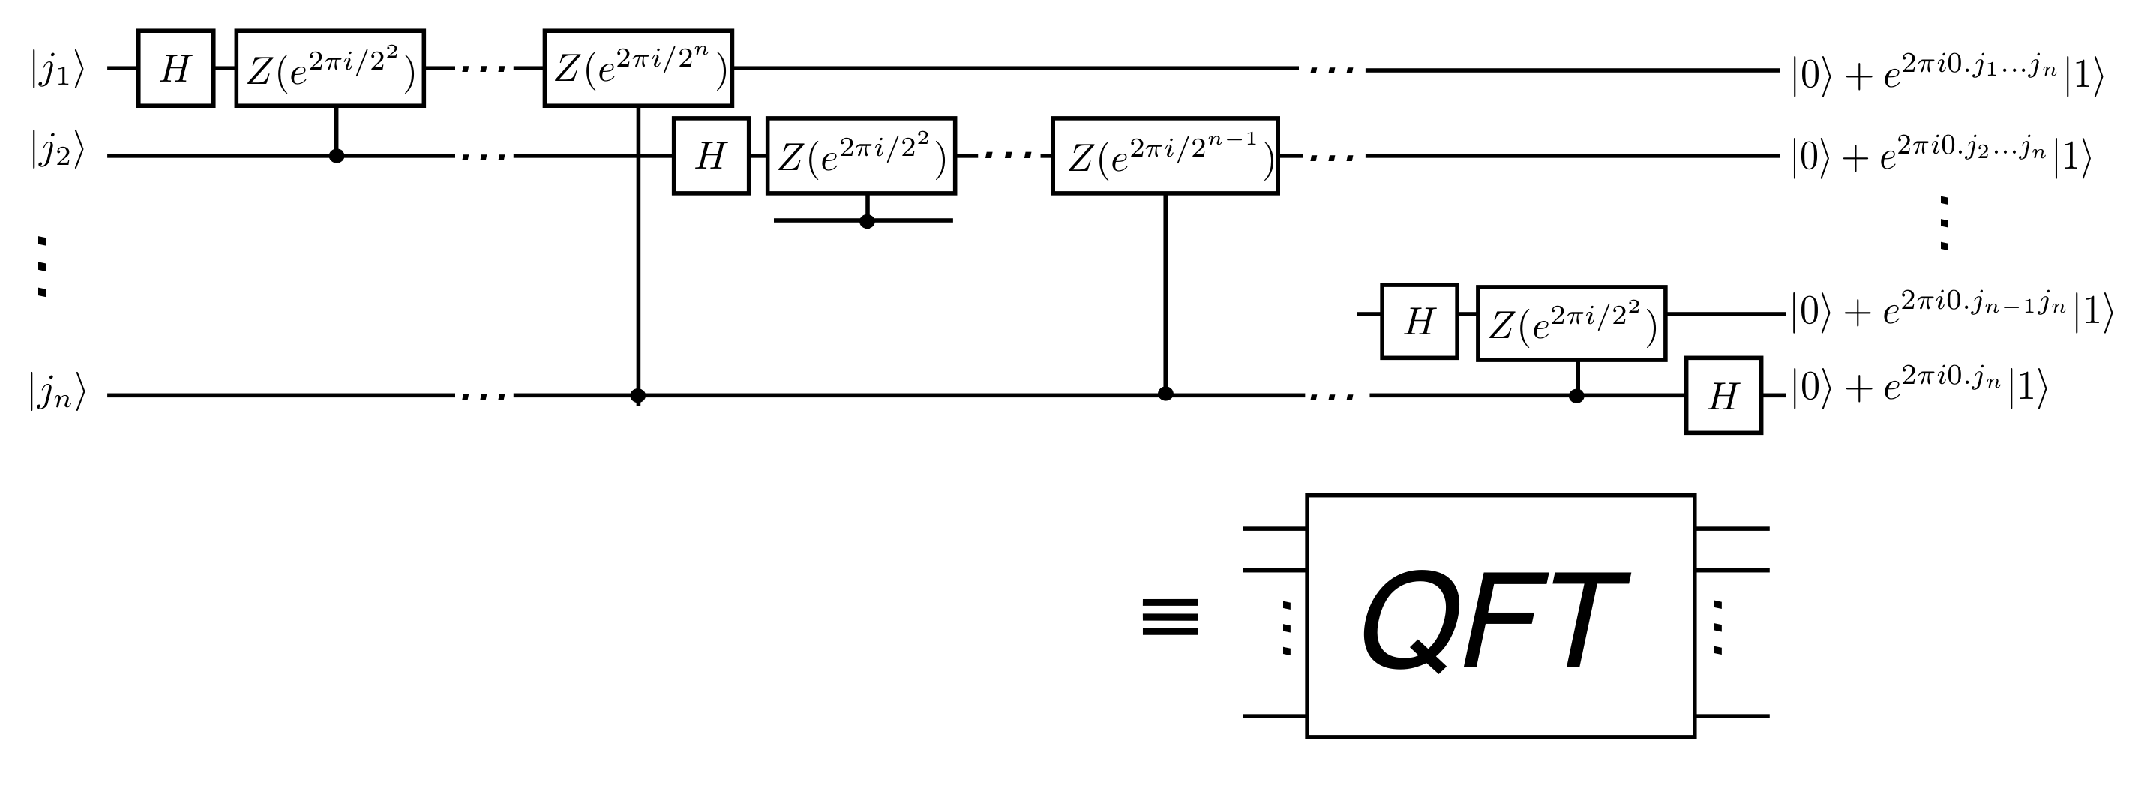
\includegraphics[width=150mm]{fig89.eps}
\end{center}
Then, we can obtain the phase $\phi = (2\pi i)0.j_1 j_2 ...j_n$ through the $Z$-basis measurements.
Note that the accuracy of the estimate is improved exponentially compared to the Hadamard test (provided that we have a polynomial size description of $\Lambda (U^{2^k})$).

Let $N$ and $x$ be co-prime integers.
The order-finding problem is about finding an order $r$ such that $x^r =1 \textrm{ mod } N$.
This problem can be solved by using the phase estimation against a unitary operator
\begin{eqnarray}
U_x = \sum _{y} |x y \textrm{ mod } N\rangle \langle y| ,
\end{eqnarray}
because we have
\begin{eqnarray}
U_x |u_s \rangle = e^{2 \pi i (s/r))} |u_s\rangle,
\end{eqnarray}
for a state
\begin{eqnarray}
|u_s\rangle = \frac{1}{\sqrt{r}}
\sum _{k=0}^{r-1} e^ {-2 \pi i (s/r) k }|x^k {\rm mod}\; N\rangle.
\end{eqnarray}
Note that we can prepare the initial state $|u_s\rangle$ randomly by using the fact that $|1\rangle= \sum _{s=0}^{r-1}|u_s\rangle$.
After estimating the phase $2 \pi i (s/r)$, the continued fraction provides $r$ with high probability.
The modular exponentiation $x^{2^k}\; \textrm{mod} \;N$ can be calculated by using the square $k$ times.
Thus we can implement controlled-$U_x^{2^k}$, $\Lambda (U_x^{2^k})$, by a polynomial number of gates.

If we randomly choose $s$, we obtain an even order $r$ with high probability.
Thus, we have $(x^{r/2}-1)(x^{r/2}+1)=0 \; {\rm mod} \; N$.
Finally, the euclidean algorithm gives us the greatest common divisor of $x^{r/2}-1$ and $N$ or $x^{r/2}+1$ and $N$, and it is a factor of $N$.
This is the so-called Shor's prime factoring algorithm.
Kitaev, who formulated the phase estimation algorithm, generalized this idea for the more general Abelian stabilizer problem~\cite{KitaevAbelian}.



\subsection{A quantum algorithm to approximate Jones polynomial}
\label{sec:JonesPoly}
\index{Aharonov-Jones-Landau algorithm}
Next we will explain Aharonov-Jones-Landau algorithm 
for approximating the Jones polynomial\index{Jones polynomial}
~\cite{AharonovJones,AharonovJonesHard},
which is an algorithmic version of 
the original proposal based on topological quantum field theory~\cite{TQFT,Witten89}.
We will show that the approximation of the Jones polynomial 
is BQP-complete;
the approximation of the Jones polynomial
can be done efficiently by using a universal quantum computer,
and inversely it is as hard as any problems (BQP) solvable by 
a universal quantum computation.
Below we will introduce the braid diagram and the braid group,
which are related to link diagrams with an appropriate closure.
A unitary representation of the braid group 
is constructed by embedding the braid group to 
the Temperley-Lieb (TL) algebra.
Using the constructed representation,
the Jones polynomial and quantum algorithm are connected.

\begin{figure}[t]
%\sidecaption
% Use the relevant command for your figure-insertion program
% to insert the figure file.
% For example, with the option graphics use
\centering
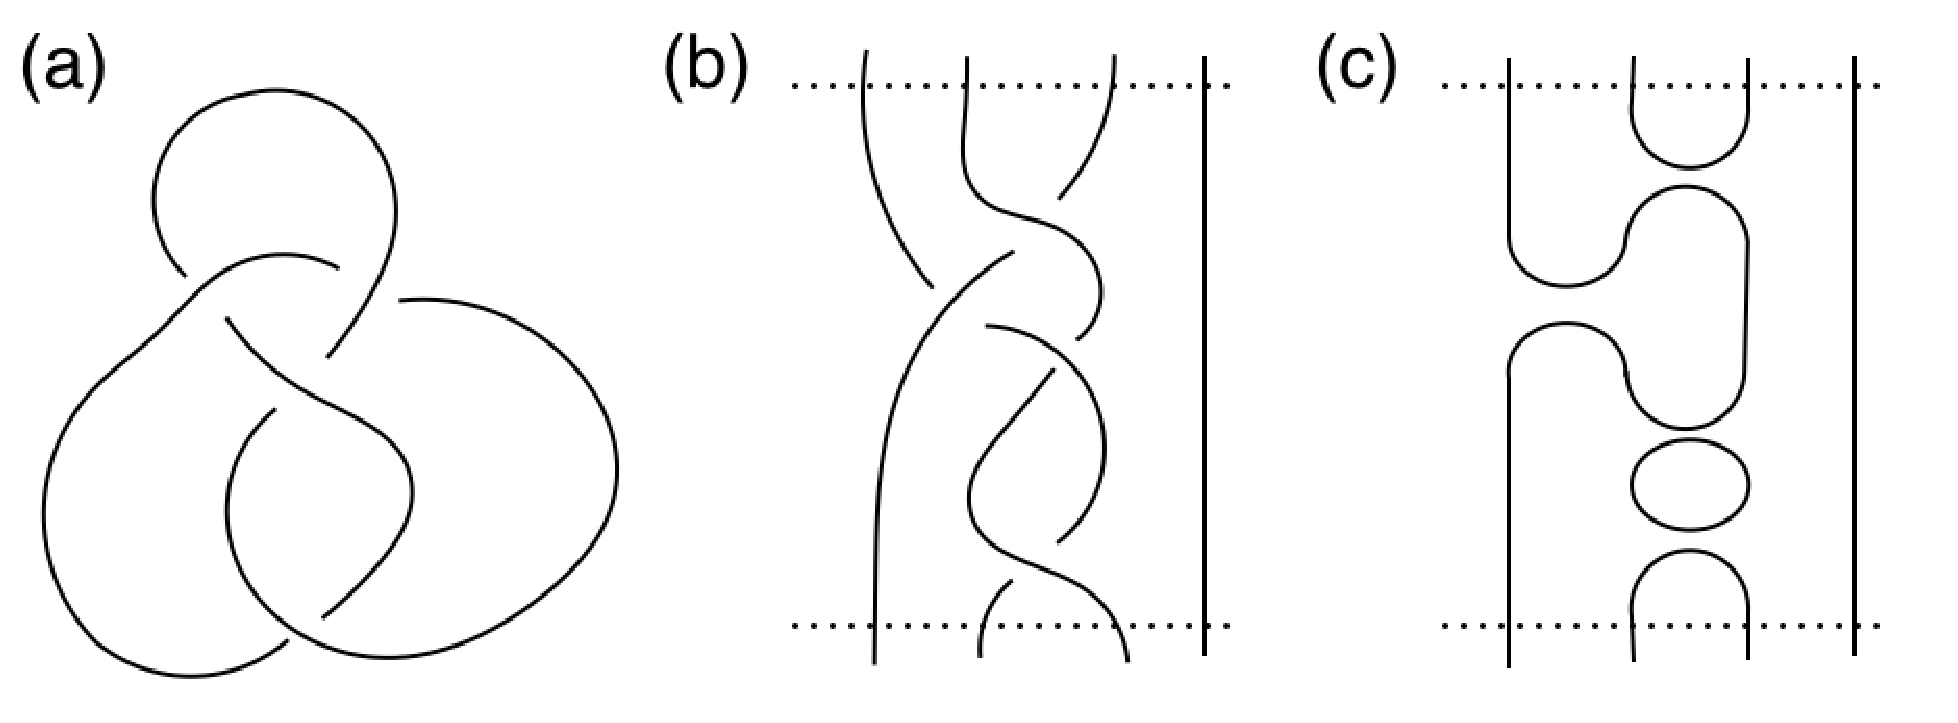
\includegraphics[width=110mm]{fig122.eps}
%
% If not, use
%\picplace{5cm}{2cm} % Give the correct figure height and width in cm
%
\caption{(a) A link diagram. (b) A braid diagram. (c) A tangle diagram.}
\label{fig122}       % Give a unique label
\end{figure}
\index{Jones polynomial}
Let us first define the Jones polynomial.
The Jones polynomial is an invariant of 
a link, that is, closed loops 
in a 3D space, which are tangled in general~\cite{Lickorish97}.
It is convenient to describe the link
on a 2D projected space as shown in Fig.~\ref{fig122} (a),
which we call a link diagram.
Specifically two links are equivalent 
if two link diagrams can be transformed into each others 
under the Reidemeister moves:
\begin{center}
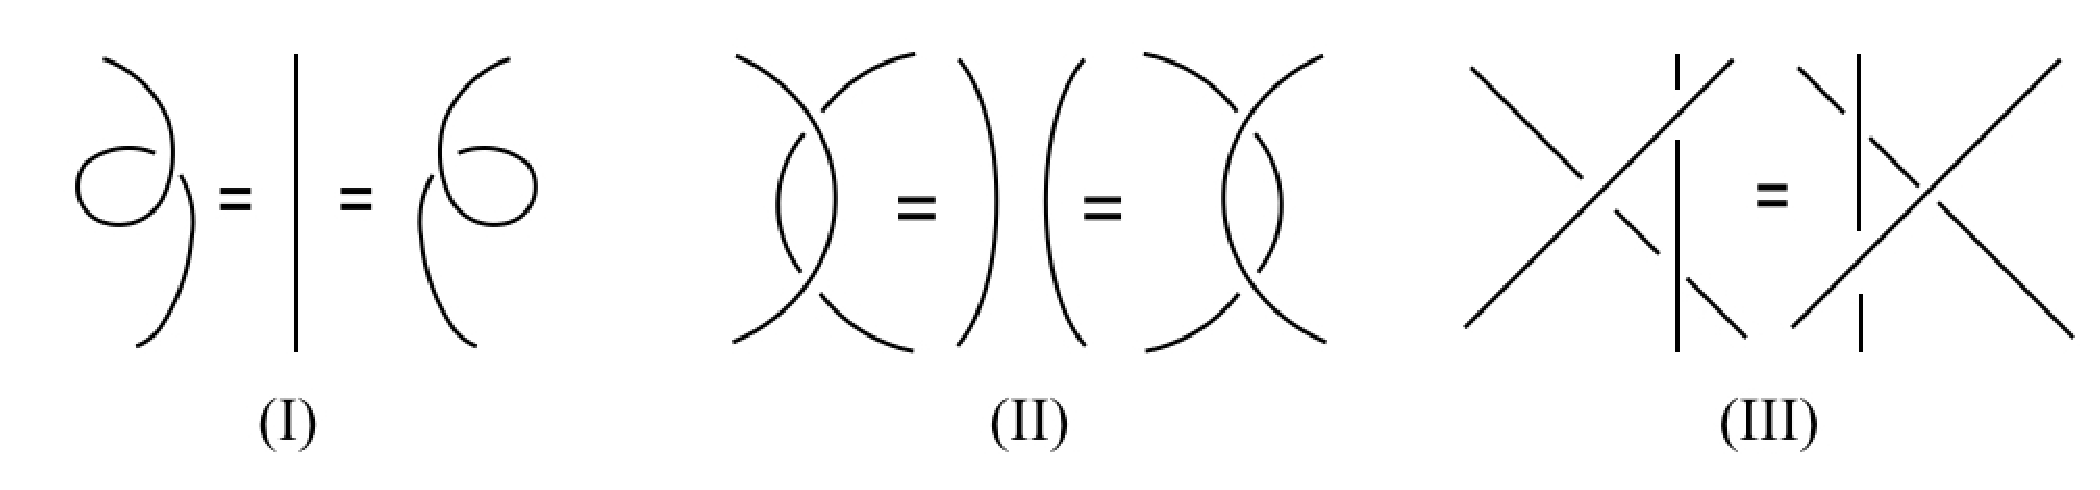
\includegraphics[width=120mm]{fig121.eps}
\end{center}
which appropriately reflect the continuous deformations in the 3D space.
The Jones polynomial is calculated from 
a directed link diagram $L$ as follows:
(i) Smooth each crossing \crosA in two ways 
$\{$\updow,\lefri $\}$.
Let $s$ be the resultant diagram consisting of 
closed loops with no crossing, which we call a state.
(ii) For each state $s$, we assign a weight 
\begin{eqnarray}
W(s) = A^{s^{+}- s^{-}} d^{|s|-1},
\end{eqnarray}
where $d=-(A^2+A^{-2})$ is a complex constant called a loop value,
$|s|$ is the number of the crossing,
and $s^{+}$ and $s^{-}$ are the number of smoothings by \updow and \lefri,
respectively.
By taking the summation over all states,
the Kauffman bracket $\langle L \rangle$ of the link $L$ is defined:
\begin{eqnarray}
\langle L \rangle = \sum _{s} W(s).
\end{eqnarray}
\index{Kauffman bracket}
The Jones polynomial is defined 
as a function of $t=A^{-4}$ by 
multiplying a factor to the Kauffman bracket: 
\begin{eqnarray}
V_L(t) = (-A)^{3 \omega (L)} \langle L \rangle,
\end{eqnarray}
where the writhe $\omega (L)$ of the link $L$ is
defined as the number of \crosA type crossings  minus 
that of \crosB type. 
It is easy and a good exercise to confirm that the Jones polynomial is invariant 
under the Reidemeister moves based on the above definition~\cite{Lickorish97}.

\index{braid group}
Let $B_n$ be a braid group 
consisting of the braid diagrams
of $n$ strands, where two endpoints of each strand
are tied at the top and bottom, respectively
as shown in Fig.~\ref{fig122} (b).
The multiplication of two braids $b_1$ and $b_2$
are defined by connecting the bottom and top endpoints 
of two braid diagrams as shown in Fig.~\ref{fig124} (a).
The braid group $B_n$ is generated 
by $n-1$ generators $\{ \sigma _i \}$
subject to
\begin{eqnarray}
&&\sigma _i \sigma _j  = \sigma _j \sigma _i \textrm{ for } |i-j|\geq 2
\\
&&\sigma _i \sigma _{i+1} \sigma _i = \sigma _{i+1}\sigma _i \sigma _{i+1}.
\end{eqnarray}
The generator $\sigma _i$ corresponds to 
the braid diagram with only one crossing of $i$th and $i+1$th strands
as shown in Fig.~\ref{fig124} (b).
\begin{figure}[t]
\centering
%\sidecaption
% Use the relevant command for your figure-insertion program
% to insert the figure file.
% For example, with the option graphics use
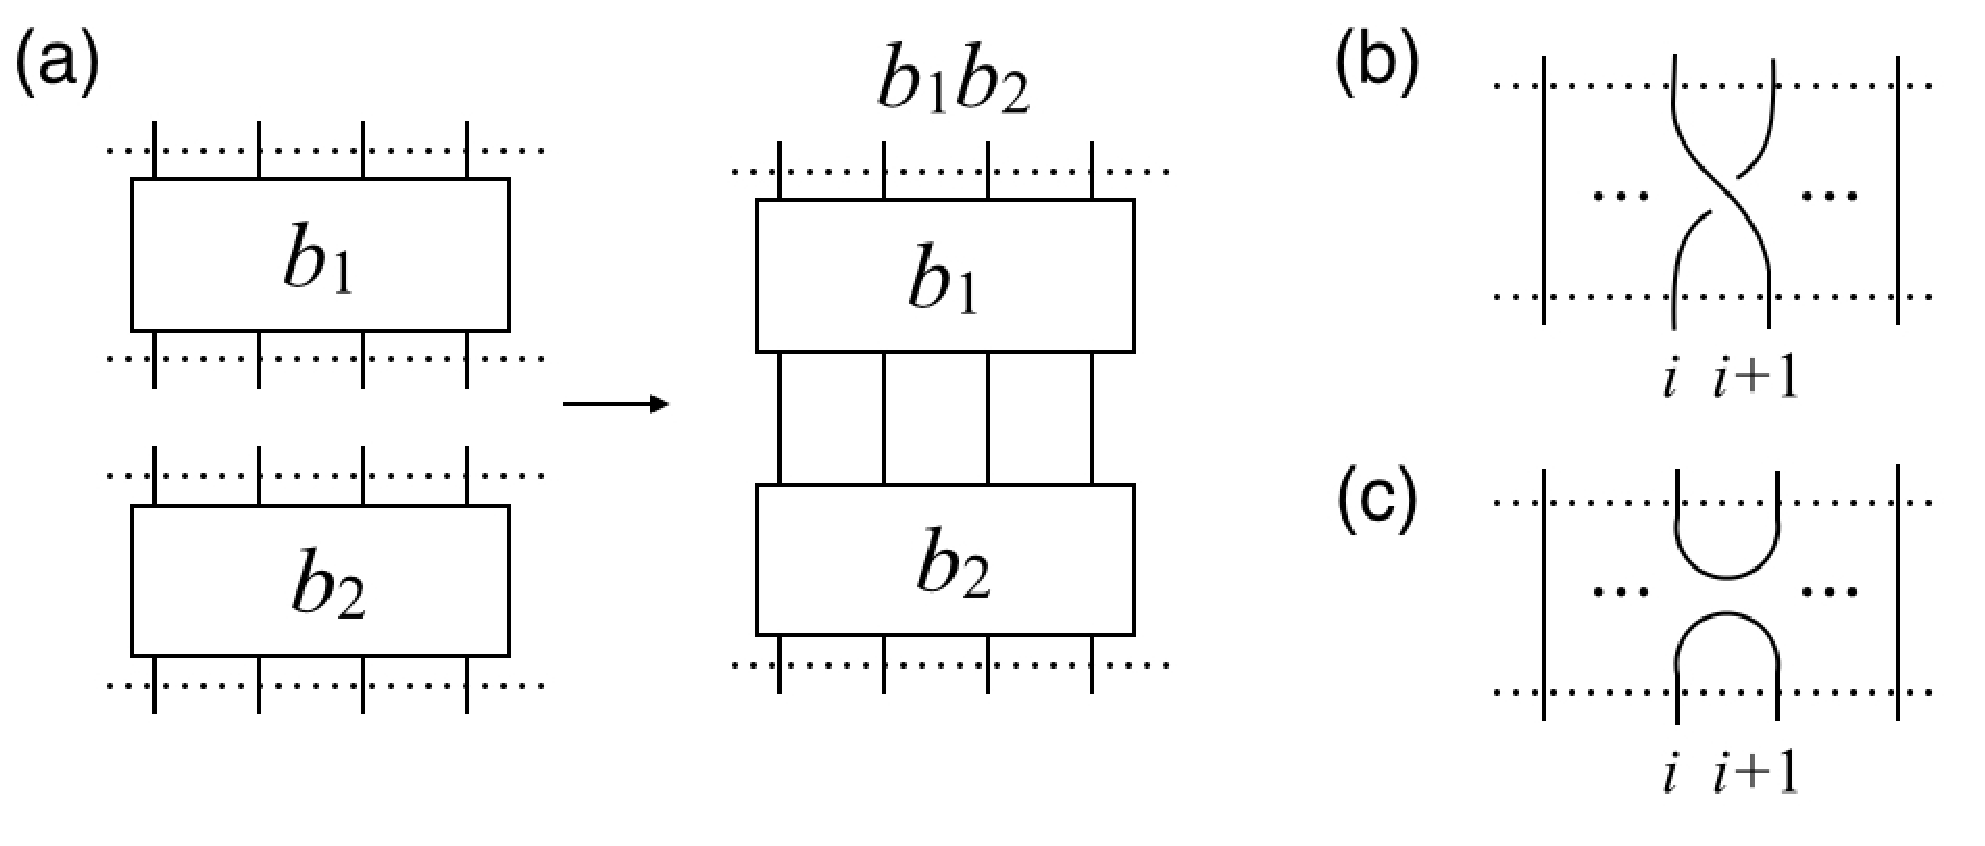
\includegraphics[width=120mm]{fig124.eps}
%
% If not, use
%\picplace{5cm}{2cm} % Give the correct figure height and width in cm
%
\caption{(a) A multiplication for two braid diagrams $b_1$ and $b_2$. (b) The generator $\sigma _i$ of the braid group. (c) The generator $E_i$ of 
the TL algebra.}
\label{fig124}       % Give a unique label
\end{figure}
Then, the latter equality is nothing but the 
Reidemeister move III.
By introducing an appropriate closure,
which closes the endpoints of the strands,
a braid diagram is related to a link diagram
as we will see later.

In order to construct a unitary representation of $B_n$,
we embed it into the Temperley-Lieb (TL) algebra $TL_n(d)$~\cite{TLalgebra}
on tangle diagrams with no crossing as shown in Fig.~\ref{fig122} (c).
\index{Temperley-Lieb (TL) algebra}
Similarly to the previous case,
$TL_n(d)$ is generated by a set of generators $\{E_1,...,E_{n-1}\}$
subject to
\begin{eqnarray}
&&E_i E_j = E_j E_i \textrm{ for } |i-j | \geq 2,
\\
&&E_i E_{i\pm1} E_i =  E_i,
\\
&&E_i^2=d E_i.
\end{eqnarray}
The generator $E_i$
corresponds to $\cup$ and $\cap$ for the $i$th and $(i+1)$th strands
as shown in Fig.~\ref{fig124} (c).
The braid group is embedded into the TL algebra by
\begin{eqnarray}
\sigma _i = A E_i + A^{-1} \mathbf{1}.
\label{eq:BraidTL}
\end{eqnarray}

\begin{figure}[t]
\centering
%\sidecaption
% Use the relevant command for your figure-insertion program
% to insert the figure file.
% For example, with the option graphics use
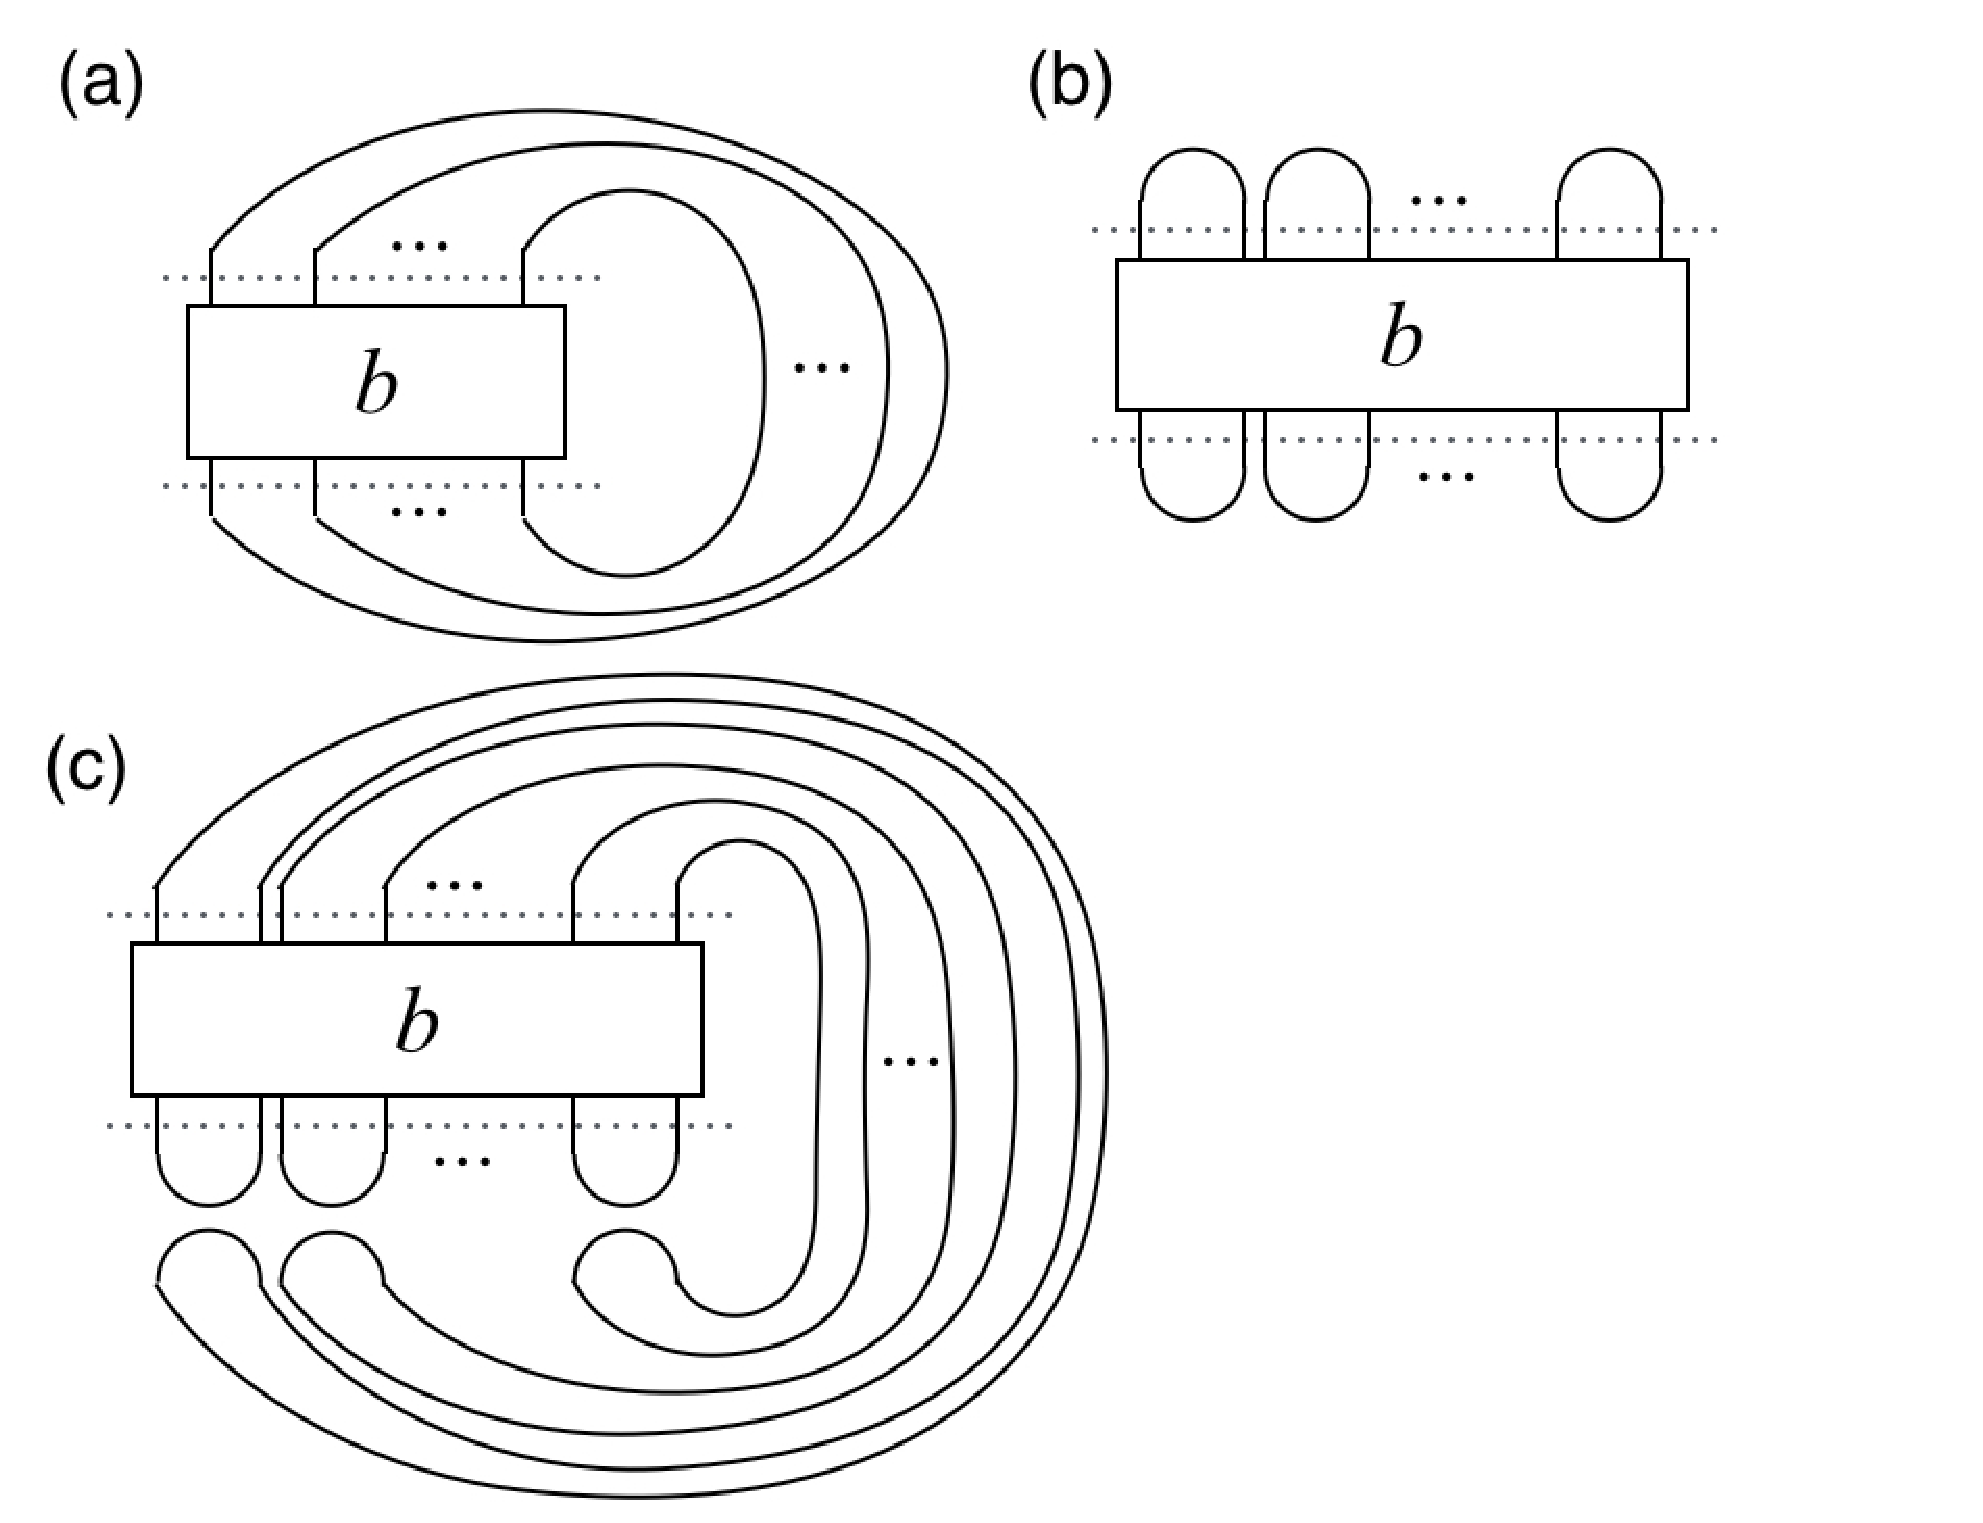
\includegraphics[width=120mm]{fig123.eps}
%
% If not, use
%\picplace{5cm}{2cm} % Give the correct figure height and width in cm
%
\caption{(a) The Markov trace closure for the braid $b$. (b) The plat closure 
for the braid $b$. (c) The plat closure 
is deformed into the Markov trace closure.}
\label{fig123}       % Give a unique label
\end{figure}
In order to relate the braid diagram 
and the Jones polynomial,
we employ a Markov trace closure on the tangle diagram as shown in Fig.~\ref{fig123} (a).
The Markov trance closure denoted by mtr has the following property: 
\begin{eqnarray}
&&{\rm mtr} (\mathbf{1})=1,
\\
&&{\rm mtr} (AB)={\rm mtr} (BA) \textrm{ for } A,B \in TL_n(d),
\\
&&{\rm mtr} (A) = d{\rm mtr} (A E_{n-1}) \textrm{ for }
A \in TL_{n-1}(d).
\end{eqnarray}
Now the representation of 
the braid group and the Jones polynomial are related.
Eq. (\ref{eq:BraidTL}) corresponds to 
superposition of two smoothings $\{$\updow,\lefri$\}$ 
of a crossing $\crosA$.
More precisely,
let $\rho$ and $\tilde \rho$ be a representation of the TL algebra 
and an induced representation 
of the braid group, respectively.
Moreover, the matrix trace 
has the same property as the Markov trace closure.
Thus,
for a given braid diagram $b$, we have
\begin{eqnarray} 
V_{b^{{\rm mtr}}}(A^{-4}) =  \Delta{\rm Tr}[\tilde \rho (b)] ,
\end{eqnarray}
where $b^{\rm mtr}$ is a link diagram 
generated from the braid diagram $b$ with the Markov trace closure,
and $\Delta _{mtr}= (-A)^{3 \omega (b^{\rm mtr})}d^{n-1}$.

Let us construct 
a representation of the TL algebra,
the so-called path-model representation.
\index{path-model representation}
Suppose $G$ is a one-dimensional graph with $k$ vertices
labeled by $1,...,k$ from left to right and $k-1$ edges.
We consider an $n$ step walk on $G$ starting from the left endpoint.
Let $p=(v_1,...,v_n)$ be a path of such an $n$ step walk,
where $v_1=1$ and $v_j =0$ and $=1$ mean moving to the left and right neighboring vertices,
respectively.
Then we define a Hilbert space $\mathcal{H}_{n,k}$ 
spanned by all possible paths as a basis $\{ |p\rangle\}$.
For each generator $E_i$, we define 
its representation $\Phi_i =\rho(E_i)$ on $\mathcal{H}_{n,k}$
as follows:
\begin{eqnarray}
\Phi _i | ... v_{i-1} 00 v_{i+1}...\rangle &=& 
0,
\\
\Phi _i | ... v_{i-1} 01 v_{i+1}...\rangle &=& 
\frac{\lambda_{z_i -1}}{\lambda_{z_i}}| ... v_{i-1} 01 v_{i+1}...\rangle+
\frac{\sqrt{\lambda_{z_i +1} \lambda_{z_i -1}}}{\lambda_{z_i}}
| ... v_{i-1} 10 v_{i+1}...\rangle,
\nonumber \\
\\
\Phi _i | ... v_{i-1} 10 v_{i+1}...\rangle &=&
\frac{\lambda_{z_i +1}}{\lambda_{z_i}}| ... v_{i-1} 10 v_{i+1}...\rangle+
\frac{\sqrt{\lambda_{z_i +1} \lambda_{z_i -1}}}{\lambda_{z_i}}
|... v_{i-1} 01 v_{i+1}...\rangle,
\nonumber \\
\\
\Phi _i |... v_{i-1} 11 v_{i+1}...\rangle &=& 0,
\end{eqnarray}
where $z_i \in \{1,...,k\}$ is the label of the vertex at the $i$th step
and $\lambda _j = \sin( j\theta)$ with $\theta =\pi  / k$. 
The representation $\tilde \rho (\sigma _i)=A\Phi _i +A^{-1} \mathbf{1}$ 
for the braid group $B_n$ is induced
by $\rho$.
It is easy to confirm that,
with $A=ie^{-i \theta /2}$ and $d=2\cos\theta$,
the representation $\rho$ is hermitian for all $E_i$, and hence
the induced representation $\tilde \rho$ is unitary.
Since $\rho (\sigma _i)$ is a unitary operator
acting on the neighboring two-qubit,
a multiplication of such unitary operators
can be implemented by using universal quantum computer.
Since, by using the Hadamard test in Sec.~\ref{sec:HadamardTest},
we can evaluate the Jones polynomial $V_{b^{\rm mtr}}(A^{-4})$
with an additive error $\Delta 2^{n} \epsilon$
taking ${\rm poly}(n,m,k,1/\epsilon)$ overhead,
where $m$ is the number of the crossing.

The approximation scale is further improved 
by considering another closure, the so-called plat closure
as shown in Fig.~\ref{fig123} (b).
We deform the link diagram obtained by the plat closure
to another link diagram obtained 
by the Markov trace closure as shown in Fig.~\ref{fig123} (c),
Then, we have $\cup$ and $\cap$ for all strands.
In this case, the support of $\rho (b)$ 
is only on $|10101...\rangle$,
which allows us to replace the matrix trace 
as follows:
\begin{eqnarray}
V_{b^{\rm plt}}(A^{-4}) = \Delta_{\rm plt} 
\langle 10101...| \rho (b) | 10101...\rangle,
\end{eqnarray}
where $b^{\rm plt}$ is a link generated from 
the braiding $b$ with the plat closure
and $\Delta _{\rm plt} = (-A)^{3 \omega (b^{\rm plt})}d^{n/2-1}$.
(Note that for each $\rho(E_i)$ of $n/2$ $\cup$s and $\cap$s, 
a factor ${\lambda_{2}/\lambda_{1}} = d$ is substituted.)
Again using the Hadamard test,
we can estimate $V_{b^{\rm plt}}(A^{-4})$ 
with an additive error $\Delta _{\rm plt} \epsilon$
taking ${\rm poly}(n,m,k,1/\epsilon)$ overhead.

Finally, we show that the approximation of the Jones polynomial 
with an additive error $\Delta _{\rm plt} \epsilon$ is BQP-hard.
Unfortunately, the computational basis defined by the path $p=(v_1,...,v_n)$
is inappropriate for this purpose,
since the $n$-step walks cannot span the whole $2^n$-dimensional Hilbert space.
Instead, we employ the four-step encoding~\cite{wocjan06}, 
where the computational basis states are defined by the following 
two four-steps:  
\begin{eqnarray}
|\bar 0 \rangle \equiv |1100\rangle, \;\;\; |\bar 1 \rangle 
\equiv |1010\rangle.
\end{eqnarray}
The space $\mathcal{H}_{4n,k}$ spanned by the $4n$-step walks
can support the whole $2^n$-dimensional space for $\{ |\bar 0 \rangle , |\bar 1\rangle \}^{\otimes n}$.
The dimension of the space spanned by the 8-step walks
starting from vertex 1 ending at vertex 1
is 14. Thus the unitary representation $\rho$ 
of the braid group $B_8$
results in unitary operators in $SU(14)$.
If they are dense in $SU(14)$,
we can approximate an arbitrary unitary operator in $SU(4)$ spanned by two four-step encoded qubits
by using the Solovay-Kitaev algorithm~\cite{AharonovJonesHard},
which are enough to implement universal quantum computation.
The density is achieved by $k>4$ and $k\neq 6$.
For such a parameter, 
the approximation of the Jones polynomial with an additive 
error $\Delta _{\rm plt} \epsilon$ is enough to solve 
a BQP-complete problem.

The approximation of the Jones polynomial 
can be done by universal quantum computer
and also is enough to solve the problems solvable by 
universal quantum computer. 
Thus the approximation of the Jones polynomial is a 
BQP-complete problem~\cite{AharonovJones,AharonovJonesHard}.
The AJL algorithm for approximation of the Jone polynomial 
was extended for the Tutte polynomial in Ref.~\cite{AharonovTutte},
where the Solovay-Kitaev algorithm for non-unitary linear operators 
was developed.


\section{Quantum noise}
Quantum coherence, one of the essential properties of quantum systems, is quite fragile against noise, due to interactions between the system and the environment.
Suppose that the system $S$ of interest interacts via a unitary operation $U$ with the environment $E$, where the system and environment are initially uncorrelated. 
The reduced density matrix $\rho' _S$ of the system after the interaction is calculated to be
\begin{eqnarray}
\rho' _S   = {\rm Tr}_{E} 
\left[U (\rho_{S} \otimes \rho _{E})U^{\dag} \right].
\end{eqnarray}
Using a spectral decomposition of the initial state in the environment, $\rho _{E} = \sum _{k} p_k |e_k \rangle \langle e_k |$, we obtain a map of the system $S$:
\begin{eqnarray}
\rho'_S = \sum _{(k',k)} K_{(k',k)} \rho _S K_{(k',k)}^{\dag},
\end{eqnarray}
where 
\begin{eqnarray}
K_{(k,k')} = \sqrt{p_k}\langle e_k' | U |e_k \rangle.
\end{eqnarray}
This map satisfies 
\begin{eqnarray}
\sum _{k}K_{(k',k)}^{\dag} K_{(k',k)} &=& 
p_k \langle e_k | U^{\dag} |e_k' \rangle 
\langle e_k' | U^{\dag} |e_k \rangle
\nonumber \\
&=& I_S,
\end{eqnarray}
where $I_S$ is the identity operator in the system $S$.

In general, a map of a quantum state is given as a completely-positive-trace-preserving (CPTP) \index{completely-positive-trace-preserving (CPTP)} map $\mathcal{E}$, subject to
\begin{itemize}
	\item ${\rm Tr} [\mathcal{E}  \rho ] =1$ for any density matrix $\rho$ (preservation of probability)
	\item $\mathcal{E}(\sum _{i} q_i \rho _i ) = \sum _i q_i \mathcal{E}\rho_i$ (convex linear map)
	\item $\mathcal{I}_{A} \otimes \mathcal{E}_S (\rho_{AS}) \geq 0$ (complete positivity) for an arbitrary ancilla system $A$ and density matrix $\rho _{AS}$ on the composite system $AS$.
\end{itemize}
Such a CPTP map can always be written by Kraus operators\index{Kraus operators} $\{ K_k\}$~\cite{NielsenChuang}:
\begin{eqnarray}
\mathcal{E} \rho = \sum _{k=1}^{M} K_{k} \rho K_{k}^{\dag}.
\end{eqnarray}

Under the Born-Markov (with rotating-wave) approximation, the time evolution of a two-level system coupled with an environment is given by a master equation of the Lindblad form~\cite{Breuer}:
%
\begin{eqnarray}
\dot \rho  (t)
&=& -  \frac{\gamma _{+}}{2} \bigl[ \sigma _{-}\sigma _{+} \rho(t) + \rho (t) \sigma _{-} \sigma _{+} - 2 \sigma _{+} \rho (t) \sigma _{-} \bigr]
 \nonumber \\
 &&  -  \frac{\gamma _{-}}{2} \bigl[ \sigma _{+}\sigma _{-} \rho(t) + \rho (t) \sigma _{+} \sigma _{-} - 2 \sigma _{-} \rho (t) \sigma _{+} \bigr]
 \nonumber \\
 &&  -  \frac{\gamma _{0}}{2} \bigl[ \sigma _{z} \rho(t) + \rho (t) \sigma _{z} - 2 \sigma _{z} \rho (t) \sigma _{z} \bigr]
 \equiv \mathcal{L} \rho (t),
\end{eqnarray}
%
where $\sigma _{+} = |0\rangle \langle 1|$, $\sigma _{-} = |1\rangle \langle 0|$ and $\gamma _{\alpha}$ ($\alpha = 0, +,-$) are the decay rates of the decay channels.
One can easily find the eigenoperators of the Lindblad super-operator. 
These eigenoperators form the damping basis \cite{Briegel93}:
%
\begin{eqnarray}
\mathcal{L} \sigma _{1} &=& 
\frac{ \gamma _{+} + \gamma _{-} + 2 \gamma _{0}}{2} \sigma _{1}
\equiv \lambda _{1} \sigma _{1},
\\
\mathcal{L} \sigma _{2} &=& 
\frac{ \gamma _{+} + \gamma _{-} + 2 \gamma _{0}}{2} \sigma _{2}
\equiv \lambda _{2} \sigma _{2},
\\
\mathcal{L} \sigma _{3} &=& 
( \gamma _{+} + \gamma _{-} ) \sigma _{3}
\equiv \lambda _{3} \sigma _{3},
\\
\mathcal{L} \rho _{eq} &=& 0,
\end{eqnarray}
%
where $\rho _{eq} = (\gamma _{+} |0\rangle \langle 0| + \gamma _{-} |1\rangle \langle 1|)/ (\gamma _{+} +\gamma _{-}) \equiv (\sigma _{0} + a \sigma _{3})/2$
with $a= (\gamma_{+}-\gamma _{-})/(2\gamma _{+} +2\gamma _{-})$.
The solution of this master equation is given by the CPTP map $\mathcal{E} (t)$:
%
\begin{eqnarray}
\mathcal{E} (t) \rho = 
p_{0} (t) \rho  + \sum _{i=1,2,3}
p_{i} (t) \sigma _{i} \rho \sigma _{i}
+ f(t) ( \sigma _{3} \rho + \rho \sigma _{3} - i \sigma _{1} \rho \sigma _{2} + i \sigma _{2} \rho \sigma _{1}),
\nonumber \\
\label{eq:noisemap}
\end{eqnarray}
%
where
%
\begin{eqnarray}
p_{0}(t) &=& \frac{1}{4} ( 1+ e ^{-\lambda _{1} t} + e^{-\lambda _{2} t} + e^{-\lambda _{3} t}),
\\
p_{1}(t) &=& \frac{1}{4} ( 1+ e ^{-\lambda _{1} t} - e^{-\lambda _{2} t} - e^{-\lambda _{3} t}),
\\
p_{2}(t) &=& \frac{1}{4} ( 1- e ^{-\lambda _{1} t} + e^{-\lambda _{2} t} - e^{-\lambda _{3} t}),
\\
p_{3}(t) &=& \frac{1}{4} ( 1- e ^{-\lambda _{1} t} - e^{-\lambda _{2} t} + e^{-\lambda _{3} t}),
\\
f(t) &=& \frac{a}{4}(1- e^{- \lambda _{3} t}).
\end{eqnarray}
%
If we consider a high temperature case (i.e., $a \rightarrow 0$), Eq. (\ref{eq:noisemap}) can be rewritten as
%
\begin{eqnarray}
\mathcal{E} (t) \rho = \left[1-   p_{1}(t) - p_{2}(t) - p_{3}(t) \right]   \rho  + \sum _{i=1}^{3}  p_{i}(t) \sigma _{i} \rho \sigma _{i}.
\label{StochasticPauli}
 \end{eqnarray}
 %
Hence, the CPTP map can be viewed as a stochastic Pauli error with probabilities $p_{i}(t)$.
In general, noise cannot be written by a stochastic Pauli error.
However, by performing an appropriate operation, one can depolarize the CPTP map into a stochastic Pauli error as a standard form, where the noiseless part of the evolution is not altered~\cite{Dur05}.
Otherwise, the Pauli basis measurements can collapse the CPTP map into a stochastic Pauli error, as we will see later.
In the rest of this book, therefore, we will consider Markovian stochastic Pauli errors only.

The fault-tolerance against more general noise has been discussed in Refs.~\cite{Aharonov97,Aharonov08,Aliferis06,Aliferis08,Aliferis09}.
If the decoherence is non-Markovian, the dynamical decoupling or quantum Zeno effect can be used to suppress the decoherence \cite{Zurek84,Vaidman96,Duan98,Viola98,Viola99,Facchi05}.
Besides, if the decoherence is spatially correlated, one can utilize a passive error-prevention scheme, the so-called {\it decoherence free subspace} (DFS), which is immune to collective noise \cite{Zanardi97,Duan97,Lidar98}.